%%%%%%%%%%%%%%%%%%%%%%%%%%%%%%%%%%%%%%%%%%%%%%%%%
\documentclass[a4paper,11pt]{article}
\pdfoutput=1 % if your are submitting a pdflatex (i.e. if you have
             % images in pdf, png or jpg format)
\usepackage{jheppub} % for details on the use of the package, please
                     % see the JCAP-author-manual
%\usepackage[english]{babel}
\usepackage{amsmath,amssymb,mathtools,tabu}
\usepackage{epsfig,epstopdf}  
\usepackage{graphicx}
\usepackage{slashed}             
\usepackage{url}
\usepackage{color,xcolor}
\usepackage{multirow}
\usepackage{multicol}
\usepackage{placeins}
\usepackage{xspace}
%\usepackage{appendix}
\usepackage{hepnames}
%\usepackage{HEPparticles}
\usepackage{comment} 
\usepackage{tocloft}
\usepackage{ptdr-definitions}
\usepackage{rotating}
\usepackage{subcaption}
%\usepackage{hyperref}
%\usepackage{cite}
\clubpenalty=1000
\widowpenalty=10000
\allowdisplaybreaks

\setlength{\bibsep}{0cm}
\bibpunct{[}{]}{,}{n}{}{,}
%\newcommand{\kt}{\ensuremath{k_{\text{T}}} \xspace}
%\newcommand{\pt}{\ensuremath{p_{\text{T}}} \xspace}
%\newcommand{\GeV}{\ensuremath{\,\text{Ge\hspace{-.08em}V}}\xspace}
%\newcommand{\TeV}{\ensuremath{\,\text{Te\hspace{-.08em}V}}\xspace}
%\newcommand{\ptmiss}{\ensuremath{\pt^\text{miss}}\xspace}
%\newcommand{\ptvecmiss}{\ensuremath{{\vec p}_{\mathrm{T}}^{\kern1pt\text{miss}}}\xspace}
%\newcommand{\fbinv} {\mbox{\ensuremath{\,\text{fb}^{-1}}}\xspace}
\newcommand{\Wprime}{\PWpr\xspace}

\newcommand{\Pb}{{{\Pqb}}\xspace}
\newcommand{\Pt}{{{\Pqt}}\xspace}
\newcommand{\Ps}{{{\Pqs}}\xspace}
\newcommand{\Pc}{{{\Pqc}}\xspace}
\newcommand{\Pd}{{{\Pqd}}\xspace}
\newcommand{\Pu}{{{\Pqu}}\xspace}
\newcommand{\PAb}{{{{\Paqb}}}\xspace}
\newcommand{\PAt}{{{{\Paqt}}}\xspace}
\newcommand{\PAs}{{{{\Paqs}}}\xspace}
\newcommand{\PAc}{{{{\Paqc}}}\xspace}
\newcommand{\PAd}{{{{\Paqd}}}\xspace}
\newcommand{\PAu}{{{{\Paqu}}}\xspace}

%\renewcommand{\Pl}{\ensuremath{\cmsSymbolFace{l}}\xspace}

%\renewcommand{\PV}{{\ensuremath{{V}}}\xspace}
\renewcommand{\PV}{{{{V}}}\xspace}
%\providecommand{\PV}{{V}\Xspace} % generic vector boson

\newcommand{\VH}{{{\PV}{\PH}}\xspace}


%%%%%%%%%%%%%%%%%%%%%%%% Abstract %%%%%%%%%%%%%%%%%%%%%%%%%%


\begin{document}
\title{SM-EFT analysis in Higgs-strahlung}

\author[a]{Suman Chatterjee,}
\emailAdd{suman.chatterjee@oeaw.ac.at}

\affiliation[a]{Institute of High Energy Physics of the Austrian Academy of Sciences (HEPHY)}

%\maketitle

\section*{Project description}

\tableofcontents

\newpage

%------------------------------------------------
\section{Science}\label{sec:sciience}

Since the start of operations in 2008, the Large Hadron Collider (LHC) at CERN has provided a data set amounting to $\approx10^{16}$ collisions that is expected to double, once more, until 2024.
During the LHC Run~2 (2015--2018), the CMS experiment~\cite{CMS_ex} collected  $136\fbinv$ of proton-proton collision data  and is now performing extensive analyses to extract the maximum knowledge on fundamental particle physics processes at the \TeV scale.
The most prominent key milestone in the LHC experiments' history is the discovery of the Higgs boson~(\PH), jointly announced by the ATLAS and CMS collaborations in 2012~\cite{Aad:2012tfa,Chatrchyan:2012ufa}.
It completed the particle content of the standard model (SM) of particle physics. 
Since then, precision measurements of the Higgs boson's mass~\cite{CMS:2017dib,CMS:2020xrn}, its charge-parity (CP) nature~\cite{CMS:2019jdw,CMS:2020cga}, its couplings to gauge bosons (\PW, \PZ, \Pgg), and other couplings have been at the center of the LHC research program with many already entering the precision regime.
% not needed->?
%third-generation fermions (\Pb, \Pt), $and second-generation leptons (\Pmu)~\cite{CMS-PAS-HIG-19-005}, among others.
\begin{comment}
\begin{itemize}
\item Discovery of Higgs boson (\PH) in 2012~\cite{Aad:2012tfa,Chatrchyan:2012ufa} resulting in the completion of the standard model (SM) of particle physics. 
This is followed by precision measurements of Higgs boson properties, such as mass~\cite{CMS:2017dib,CMS:2020xrn}, CP nature~\cite{CMS:2019jdw,CMS:2020cga}, coupling to gauge bosons, third-generation fermions, and second-generation leptons~\cite{CMS-PAS-HIG-19-005}, among others.
\item Precision measurements of processes involving electroweak gauge bosons (\PW, \PZ, \Pgg), light- and heavy-flavor quarks (\Pu, \Pd, \Ps, \Pc, \Pb, \Pt), gluons (\Pg).
\item Discovery of processes not observed previously in colliders, such as light-by-light scattering~\cite{CMS:2018erd}, single-production of a top quark in association with a \PZ boson~\cite{CMS:2018sgc}, vector boson scattering~\cite{CMS:2017fhs}, among others.
\item Constraining a large region of parameter space in models beyond the SM (BSM) constructed with extended symmetries 
constructed to explain several observed phenomena and to provide an explanation of theoretical quests.
\end{itemize}
\end{comment}
At the same time, the lack of smoking-gun evidence for resonant phenomena beyond the SM~(BSM) has discouraged many sophisticated models that were conceived to cure, at various degrees, the SM's shortcomings. Supersymmetry, a viable dark matter candidate or models with extra dimensions have not been discovered. 

Is the case, therefore, closed? 
In this proposal we argue on the contrary. In fact, the recent advent of effective field theories~(EFT)~\cite{Grinstein:1991cd,Chiu:2007dg,Passarino:2016pzb} demonstrates impressively that subtle deviations, hiding in the observables' distributions, can probe BSM phenomena at energy scales often exceeding the LHC's reach in the direct searches. 
The underlying theoretical framework is the SM effective field theory~(SM-EFT)~\cite{Jenkins:2013zja,Alonso:2013hga,Jenkins:2013wua,Englert:2014cva,Brivio:2017vri} that systematically extends the SM with operators of higher mass dimension that smoothly change the kinematic spectra.
Specifically,  SM-EFT modifications to the SM Higgs sector result in deviations that grow with the momenta of the final state particles. 
The joint production of a \PH boson and a vector boson (\VH with \PV$=\PW^{\pm},\PZ$) are particularly strongly effected, turning the highly energetic \VH final states into extremely important discovery tools for BSM phenomena. 
In addition, BSM sources of CP violation change subtle triple-correlations of angular observables that are easily lost if not targeted explicitly by means of ``interference resurrection''~\cite{Panico:2017frx}.
The latter techniques have been demonstrated in the simpler $\PW\gamma$ final states~\cite{CMS-PAS-SMP-20-005}, but the order-of-magnitude sensitivity gain for precision measurements, although proposed recently~\cite{Banerjee:2019twi}, has not been exploited experimentally in the Higgs sector. 
% FIXME Instead of the following, make a nice list of UV models you actually constrain and list them in Section 5. --> Done (added in Sec. 4)
% For example, the existence of a heavy gauge boson of mass beyond the LHC reach can manifest itself modifying {\PH}-{\PV} couplings~\cite{Appelquist:1974tg}. 
% The second most dominant mechanism of Higgs boson production at LHC is in association with a vector boson, referred to as \VH production, which involves a $s$--channel vector boson. 

To close these gaps, I propose an extensive measurement of the \PH--\PV couplings in \textcolor{red}{\VH final states}. Resurrecting the process' interference pattern and simultaneously leveraging the energy growth in the kinematic tails of the \PH, $\PW^{\pm}$, and \PZ bosons promises unique sensitivity and a wide reach to SM-EFT effects, including the CP coupling structure.
The proposed analysis includes differential cross section measurements of a number of observables never considered before.
Combining \PH boson decays to a pair of \Pb quarks with the requirement of leptonic \PV decays~(electrons or muons), leads to a high signal acceptance while suppressing the difficult hadronic backgrounds.  

% FIXME -> Methodology?
%The \VH production with \PV decaying to leptons is an ideal place to probe \PH in its dominant decay mode to a pair of \Pb quarks as the leptons can be used to select the targeted events at the trigger-level and also to reduce the multijet background from quantum chromodynamics (QCD) interaction.

% FIXME -> Research hypothesis (or maybe drop)
%The production of \PV from quark-antiquark annihilation, the associated production of \PH from \PV, and the decay of \PH to a pair of \Pb quarks are sensitive to the footprint of new physics at respective vertices, namely vector couplings, gauge couplings, and Yukawa couplings. %in $\PH \to \Pb \PAb$ decay. 
% FIXME -> I added the following information in the research hypothesis. --> Thanks!
%A number of such couplings involving the Higgs boson can be directly probed for the first time at LHC~\cite{Gupta:2014rxa}. The rest of the couplings, which could have left signatures in earlier experiments like LEP, can also be probed with better accuracy at LHC because of the increase of their impact with energy~\cite{Ellis:2014jta,Grojean:2018dqj}.

% FIXME -> Can drop, already used above.
%The \VH production also gives an unique opportunity to probe the CP-sensitivity in \PH--\PV coupling,  which can be probed using novel techniques developed very recently, known as interference resurrection~\cite{Panico:2017frx}, not explored so far in the Higgs sector. The proposal changes the scenario in the area of experimental measurements.  

The work can start with the data set alread collected during the LHC's Run~2. 
With the additional $160\fbinv$ data to be delivered by LHC in Run~3 (2022--2024), these measurements are expected to have a significant leap in precision. In the remainder of the proposal, I attempt to demonstrate these claims.


\section{Research hypothesis}
\label{sec:research_hypo}

%\subsection{Effective field theory couplings in \PV($\to$ \Pl\Pl)\PH($\to$ \Pb \PAb) production}

I assume that \TeV scale phenomena are described by the standard model effective theory (SM-EFT). 
The SM-EFT progressively includes operators of mass dimension greater than four that respect the SM symmetries~\cite{Jenkins:2013zja,Alonso:2013hga,Jenkins:2013wua,Englert:2014cva,Brivio:2017vri} and is defined by the Lagrangian
\begin{equation}
\mathcal{L}_{\text{SM-EFT}} = \mathcal{L}_{\text{SM}} +  {\sum}_{i} \frac{\text{c}_i^{\left(5\right)}}{\Lambda} \mathcal{O}_{5,i} + {\sum}_{i} \frac{\text{c}_i^{\left(6\right)}}{{\Lambda}^{2}} \mathcal{O}_{6,i} + ... \;.
\label{Eq:SMEFT}
\end{equation}
It captures all non-resonant BSM phenomena below an arbitrarily chosen energy scale $\Lambda$.
The dimensionless Wilson coefficients $\text{c}$ are used to parametrize the effects on observables, while the terms $\mathcal{O}_{5(,6),i}$ are  the operators at mass dimension 5 and 6, respectively.
The only possible dimension-5 candidate is the  Weinberg operator~\cite{PhysRevLett.43.1566}, not relevant for the phenomenology of this proposal ~\cite{Bonnet:2009ej}.
% FIXME -> let's not discuss what we don't want to discuss.
%the smallness of neutrino mass points to the relevance of this operator only at energy much higher than that relevant for LHC physics. 
% FIXME -> Too much, I think ... (hermiticity, 2010)
%The complete set of non-redundant operators at  dimension-6, except for the Hermitian conjugates, written for the first time in 2010 forms the so-called Warsaw basis~\cite{Grzadkowski:2010es}. 
The number of baryon- and lepton number conserving dimension-6 operators is 2499 when all flavor degrees of freedom are counted. There are 76 operators respecting a $\textrm{U}(3)^5$ flavor symmetry~\cite{Alonso:2013hga} among which the 12 in Table~\ref{Tab:Operators} affect the \VH process.
The operators are written in the so-called Warsaw-basis basis~\cite{Grzadkowski:2010es} and it is the central aim of this proposal to constrain their Wilson coefficients via their numerous effects on the Higgs boson production properties and decay kinematics~\cite{Hagiwara:1993qt,Ellis:2014dva,Murphy:2017omb,Baglio:2020oqu}.

\begin{table}[tph]
\caption{
The dimension-6 operators in the Warsaw basis~\cite{Grzadkowski:2010es} affecting \VH  processes.
}
\begin{center}
{\renewcommand{\arraystretch}{1.3}
\begin{tabular}{lcl|lcl}
${\cal O}^{(1)}_{Hq}$&&$i H^\dagger \overleftrightarrow{D}_\mu H \bar{q}   \gamma^\mu q$&${\cal O}_{HWB}$&&$ H^\dagger \sigma^a H W^a_{\mu\nu}B^{\mu\nu}$ \\
\rule{0pt}{4ex} ${\cal O}^{(3)}_{Hq}$&&$i H^\dagger \sigma^a \overleftrightarrow{D}_\mu H \bar{q}  \sigma^a \gamma^\mu q$ &${\cal O}_{H\tilde{W}B}$&&$ H^\dagger \sigma^a H W^a_{\mu\nu}\tilde{B}^{\mu\nu}$\\
\rule{0pt}{4ex} ${\cal O}_{Hu}$&&$i H^\dagger \overleftrightarrow{D}_\mu H \bar{u}_R  \gamma^\mu u_R$&${\cal O}_{H{W}}$&&$ |H|^2 W_{\mu\nu}{W}^{\mu\nu}$\\
\rule{0pt}{4ex} ${\cal O}_{Hd}$&&$i H^\dagger \overleftrightarrow{D}_\mu H \bar{d}_R  \gamma^\mu d_R$&${\cal O}_{H\tilde{W}}$&&$ |H|^2 W^a_{\mu\nu}\tilde{W}^{a \mu\nu}$\\
\rule{0pt}{4ex} ${\cal O}_{HD}$&&$(H^\dagger  {D}_\mu H)^*(H^\dagger  {D}_\mu H)$& ${\cal O}_{HB}$&&$|H|^2 B_{\mu\nu}B^{\mu\nu}$\\
\rule{0pt}{4ex} ${\cal O}_{H\square}$&&$(H^\dagger H) \square (H^\dagger H)$& ${\cal O}_{H\tilde{B}}$&&$|H|^2 B_{\mu\nu}\tilde{B}^{\mu\nu}$
%\hline
\end{tabular}}
\label{Tab:Operators}
\end{center}
\end{table}

The operators ${\cal O}^{(1)}_{Hq}$, ${\cal O}^{(3)}_{Hq}$, ${\cal O}^{(1)}_{Hu}$, and ${\cal O}^{(1)}_{Hd}$ introduce the 4-point interactions depicted in Fig.~\ref{fig:Feynman_digarams} (left). 
Together with ${\cal O}_{HD}$ and ${\cal O}_{HWB}$, these six operators describe all relevant \PV-fermion coupling modifications (Fig.~\ref{fig:Feynman_digarams}, middle). 
The remaining operators modify the \PH--\PV coupling, shown in Fig.~\ref{fig:Feynman_digarams} (right). 
There is also the Yukawa-type operator $H^\dagger H \bar{Q}\phi b$, which only changes the $\PH \to \Pb \PAb$ branching ratio and, thus, can be probed in an inclusive cross section measurement. 
\begin{figure*}[hbtp]
\begin{center}
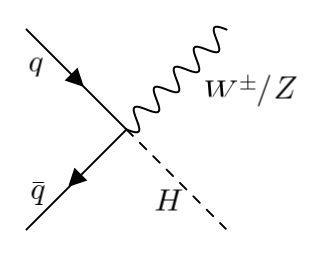
\includegraphics[width=0.3\textwidth]{Figures/Feynman_diagrams/ffVh.png}
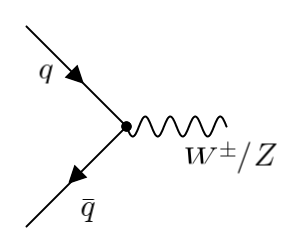
\includegraphics[width=0.3\textwidth]{Figures/Feynman_diagrams/Vff.png}
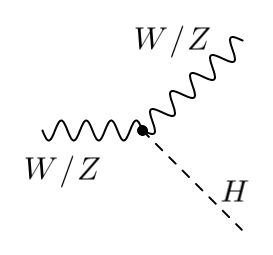
\includegraphics[width=0.3\textwidth]{Figures/Feynman_diagrams/hVV.png}
\end{center}
\caption{
Feynman diagrams for \VH production sensitive to different dimension-6 operators.
The energy growth induced by the diagrams in \VH production cross section are the following: $E^2$ (left), $E^0$ (middle), $E$ (right). 
}
\label{fig:Feynman_digarams}
\end{figure*}

%\subsection{Direct measurements of SM-EFT couplings in \PV($\to \Pl \Pl $) \PH ($\to \Pb \PAb$)}

%SM-EFT parameters can, in general, be constrained using data from the previous low-energy experiments by replacing \PH by its vacuum expectation value ($v$) in operators in Table~\ref{Tab:Operators}. For a majority of the operators at work here, which are of the form ${\PH}^2\mathcal{L}_{\text{SM}}$,
%this just corresponds to a shift of the parameters in SM Lagrangian. 
%Therefore, those can be probed directly for the first time at LHC.

The $\textrm{SU}(2)$ doublet \PH is expanded as $\begin{pmatrix} 0 \\ v+h \end{pmatrix}$, where $v$ is the vacuum expectation value  and $h$ corresponds to the physical Higgs boson.
At weak scale,  \PH is replaced by $v$ in operators in Table~\ref{Tab:Operators}, and some of them can be constrained using the existing collider results from  the LEP and the Tevatron experiments.
Nevertheless, the expected bounds from the LHC are expected to be more stringent~\cite{Ellis:2014jta,Grojean:2018dqj}.
In turn, the operators of the form ${\PH}^2\mathcal{L}_{\text{SM}}$, can be directly probed for the first time at LHC~\cite{Gupta:2014rxa}. 

The feynman diagram with four-point interaction (Fig.~\ref{fig:Feynman_digarams}, left) involves one scalar and one vector fields, each with mass dimension 1, and two fermion fields, each with mass dimension $\frac{3}{2}$.
%thus, the corresponding operator expansion has the form $\frac{v}{{\Lambda}^2} E^5$ in high energy limit.
%Therefore, the exponent in $S$-matrix, $\int L d^{4}x$, takes the form  $\sim \frac{vE}{{\Lambda}^2}$, 
Power counting with naive dimensional analysis~\cite{Manohar:1983md} implies that this causes an energy growth of $E^2$ in cross section. 
Similarly, after replacing \PH by  the diagram with the modification with fermion--\PV coupling (Fig.~\ref{fig:Feynman_digarams}, middle) 
corresponds to Lagrangian expansion of the form $\frac{v^2}{{\Lambda}^2} V_{\mu} \bar{\psi} {{\gamma}^{\mu}} {\psi}$ %\to \frac{v^2}{{\Lambda}^2} E^4$ in high energy limit
and does not that induce an energy growth in cross section. 
The operators modifying \PH--\PV coupling (Fig.~\ref{fig:Feynman_digarams}, right) give rise to terms $vh {\partial}^{\mu}{\partial}^{\nu} V_{\mu}V_{\nu}$.
%$\sim (\frac{v^2}{2}+vh+\frac{h^2}{2}) ({\partial}^{\mu}{\partial}^{\nu} V_{\mu}V_{\nu} + ...)$, 
%which goes as $\frac{vE}{{\Lambda}^2}$ in high energy limit. 
When interfering with the SM term ($\left(H^{\dagger}H\right) V^{\mu}V_{\mu}$) gives rise a linear energy growth in cross section.
%FIXME One sentence about power counting and energy growth. Then come the angles below ... --> Done
%FIXME -> Drop? Is the BSM acceptance really relevant anywhere?
%The methodology used in conventional measurements of SM-EFT operators assumes that all the object and event selection conditions have the same efficiency and acceptance for the SM and SM-EFT operators, which is known to be not the case always, and also miss important subtle effects by integrating over a number of important variables.% as will be shown in Sec.~\ref{sec:method}.
The proposed measurement will probe the operators in Table~\ref{Tab:Operators} 
using kinematic variables exhibiting energy growth and, for the first time, angular information that is sensitive to subtle interference effects.
For the latter, we exploit the techniques of Ref.~\cite{Banerjee:2019twi} and define the angles and decay planes of the \VH process as shown in Fig.~\ref{fig:HelicityFrame}.
% FIXME Here please describe concretely the angular amplitudes. Eq. 3.6 from Spannowsky, mention how these integrated to zero, and note the CP structure. --> Done 

% not only allow to disentangle energy growth induced by different operators, but also provide an unique opportunity to sense the additional sources of CP violation due to dimension-6 operators in SM-EFT.
\begin{figure*}[hbtp]
\begin{center}
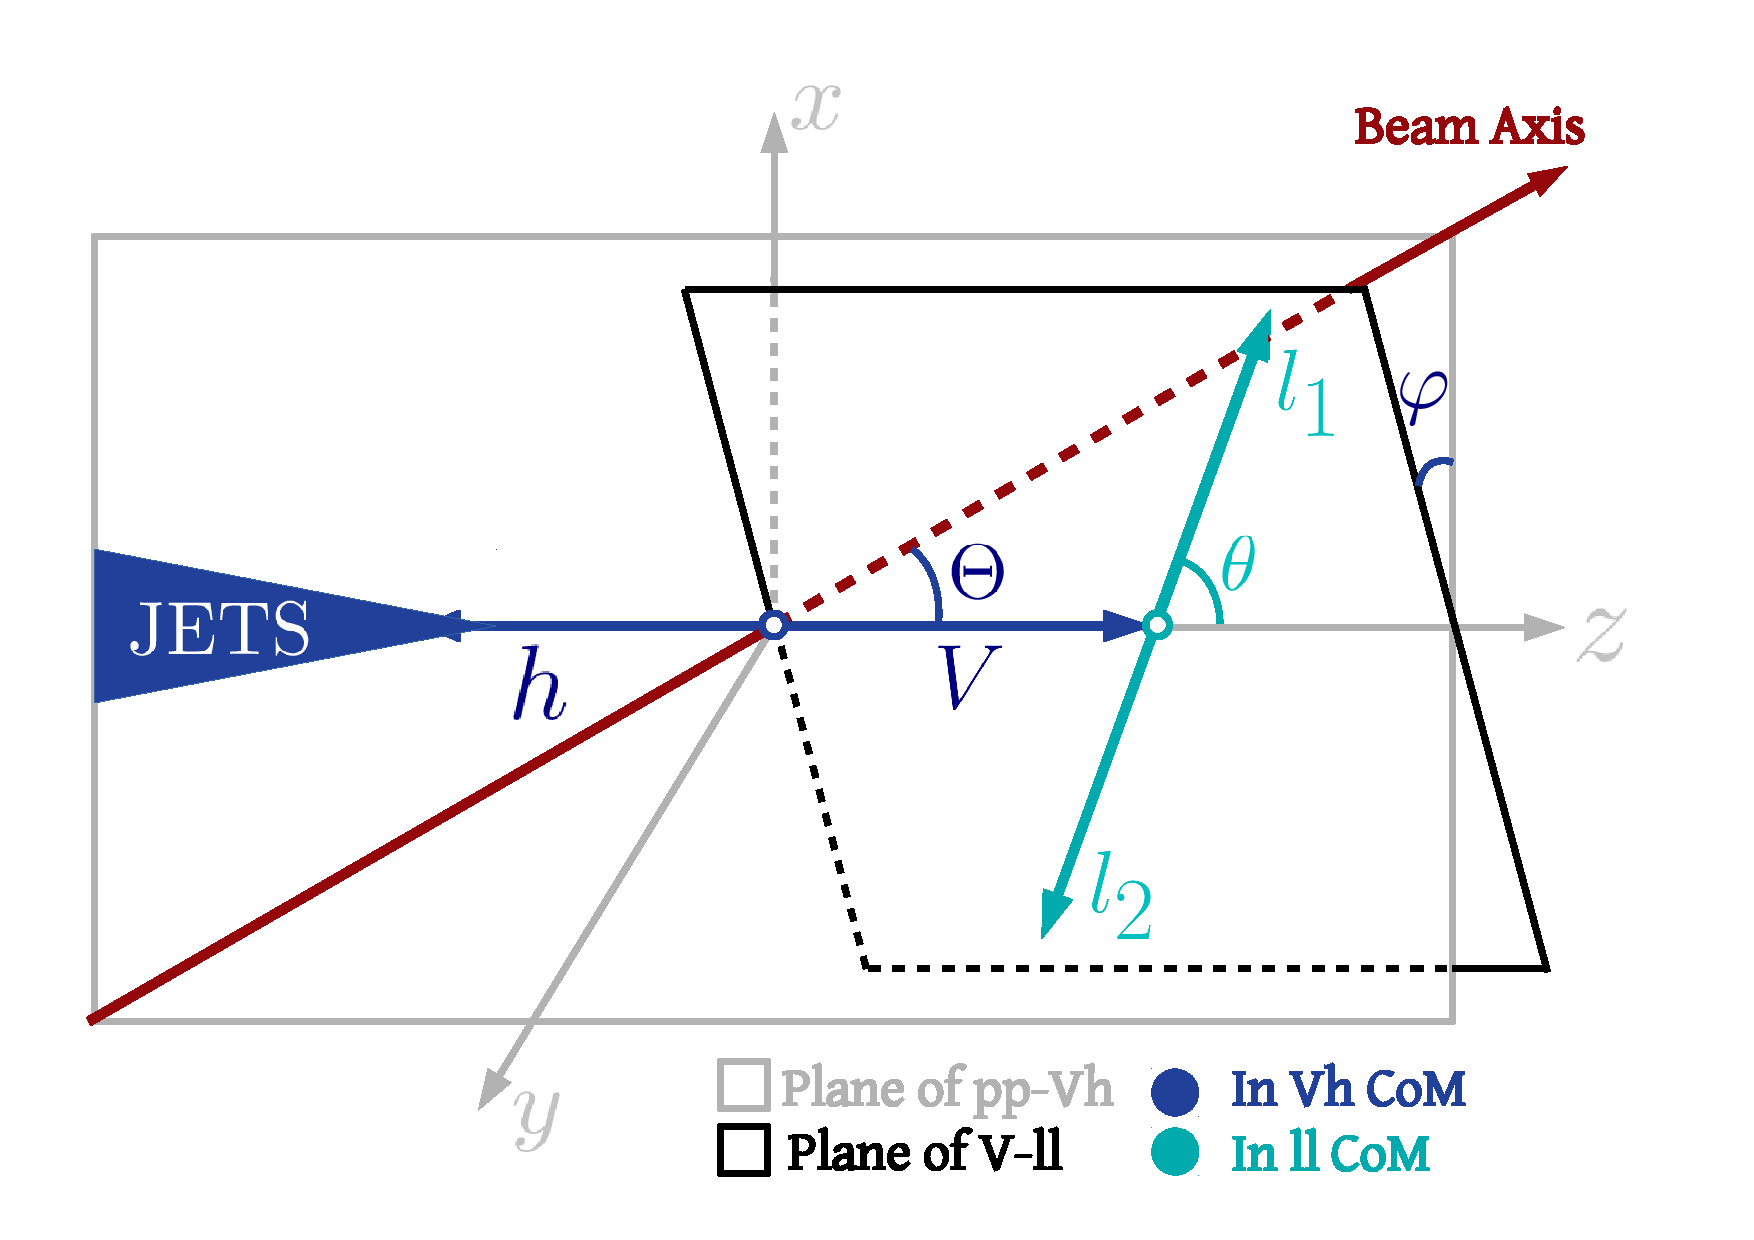
\includegraphics[width=0.75\textwidth]{Figures/LHE/TheThreeAnglesVh.pdf}
\end{center}
\caption{
Decay planes and angles in the \PV($\to \Pl \Pl$)\PH($\to \Pb \PAb$) decay. Note that $\Theta$ is defined in the $\PH\PV$ rest frame, while $\theta$ is defined in the \PV rest frame.
}
\label{fig:HelicityFrame}
\end{figure*}

The squared amplitude of \PV($\to \Pl \Pl$)\PH($\to \Pb \PAb$) production, when summing over the lepton helicities, has the following form
\begin{equation}
	|\mathcal{M} \left(\hat{s}, \Theta, \theta, \varphi \right)|^{2} = {\sum}_{i} a_i \left(\hat{s}\right) f_i \left(\Theta, \theta, \varphi \right) \ ,
\label{Eq:Amplitude}
\end{equation}
where $a \left(\hat{s}\right)$'s are functions of Wilson coefficients and the energy transfer involved in the process ($\hat{s}$) and $f$'s, functions of three angles, have the following forms with indices refering to the polarizations of the intermediate vector boson:
\begin{eqnarray}
    f_{1} = f_{LL} &=& \sin^{2}\Theta \sin^{2}\theta,{\nonumber}\\
    f_{2} = f^1_{TT} &=& \cos\Theta \cos\theta,{\nonumber}\\
    f_{3} = f^2_{TT} &=& (1+\cos^{2}\Theta)(1+ \cos^{2}\theta),{\nonumber}\\
    f_{4} = f^1_{LT} &=& \cos\varphi \sin\Theta \sin\theta,{\nonumber}\\
    f_{5} = f^2_{LT} &=& \cos\varphi \sin\Theta \sin\theta \cos\Theta \cos\theta,{\nonumber}\\
    f_{6} = \tilde{f}^1_{LT} &=& \sin\varphi \sin\Theta \sin\theta, {\nonumber}\\
    f_{7} = \tilde{f}^2_{LT} &=& \sin\varphi \sin\Theta \sin\theta \cos\Theta \cos\theta,{\nonumber}\\
    f_{8} = f_{TT'} &=& \cos^{2}\varphi \sin^{2}{\Theta} \sin^{2}{\theta},{\nonumber}\\
    f_{9} = \tilde{f}_{TT'} &=&  \sin^{2}{\varphi} \sin^{2}{\Theta} \sin^{2}{\theta}\,	.
    \label{Eq:funcs}
\end{eqnarray}
A traditional inclusive measurement integrating over $\Theta, \theta, \varphi$ makes all the terms in Eq.~\eqref{Eq:funcs}, except $f_{LL}$ and $f^2_{TT}$, vanish causing a loss of important information, which can only be reovered using a triple differential analysis with respect to all three angles.
One point to note here is that the absence of knowledge about the direction of incoming quark and anti-quark makes the terms in Eq.~\eqref{Eq:Amplitude} corresponding to $f^1_{TT}$, $f^1_{LT}$, and $\tilde{f}^1_{LT}$ vanish.

\begin{comment}
Now, the operators at Table~\ref{Tab:Operators} can also be constrained using the existing measurements in Higgs sector at LHC~\cite{CMS-PAS-HIG-19-005,ATLAS:2020fcp,ATLAS:2020jwz}. 
However, this methodology assumes that all the object and event selection conditions have the same efficiency and acceptance for the SM and SM-EFT operators, 
which is known to be not the case always. 
Also, as will be shown in Sec.~\ref{sec:method}, some important effects can be lost in traditional measurements of kinematic variables. 
Therefore, it is necessary to construct a set of observables that can extract telltale signatures of EFT operators without any loss of information. 
Also, the impact of all the conditions applied at the analysis level needs to be checked for the operators involved. 
These goals can only be achieved in a dedicated measurement as proposed here.
\end{comment}


\section{Objectives}
\label{sec:objective}

\begin{figure*}[t]
\begin{center}
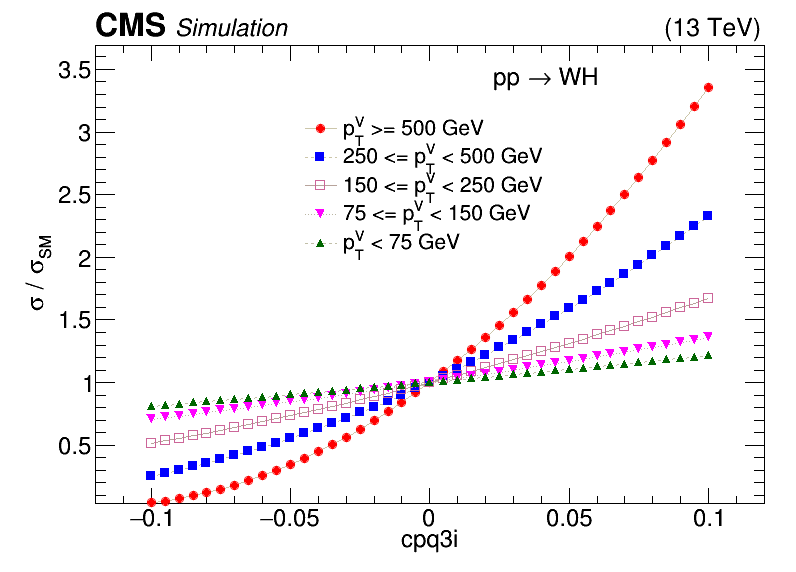
\includegraphics[width=0.321\textwidth]{Figures/LHE/WH/Canv_cpq3i.png}
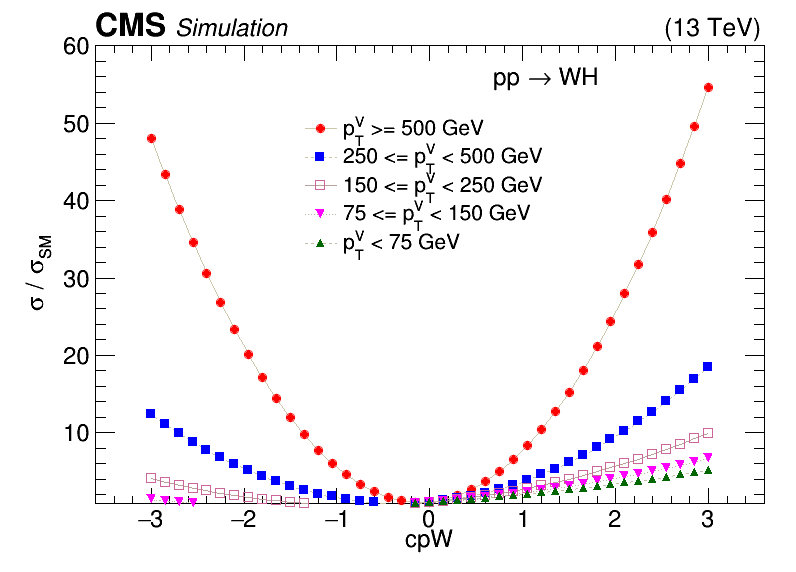
\includegraphics[width=0.321\textwidth]{Figures/LHE/WH/Canv_cpW.png}
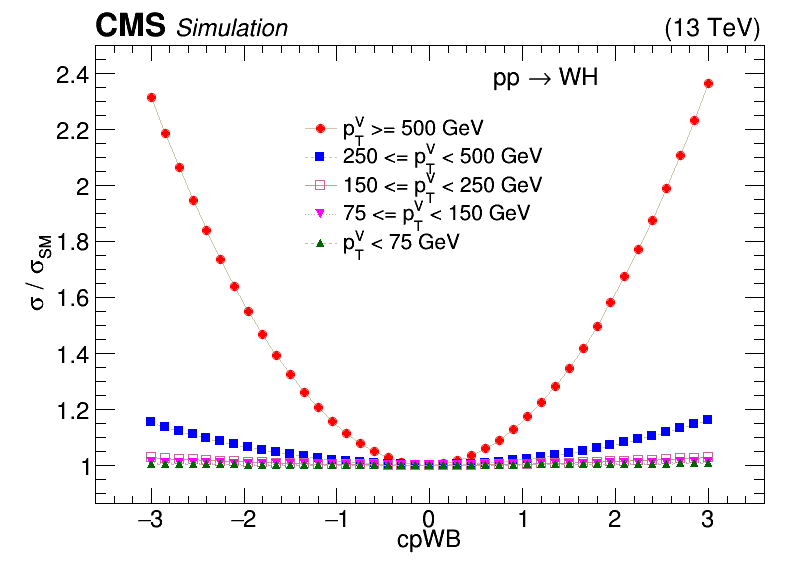
\includegraphics[width=0.321\textwidth]{Figures/LHE/WH/Canv_cpWB.png}
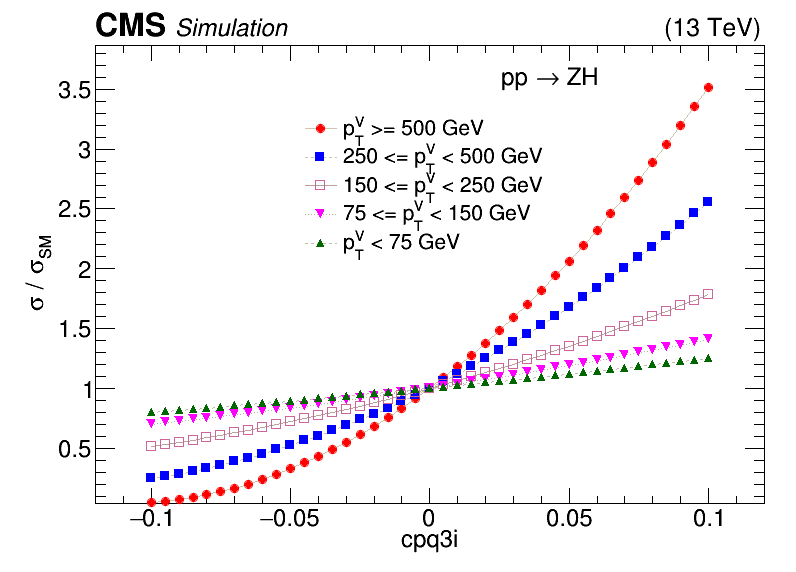
\includegraphics[width=0.321\textwidth]{Figures/LHE/ZH/Canv_cpq3i.png}
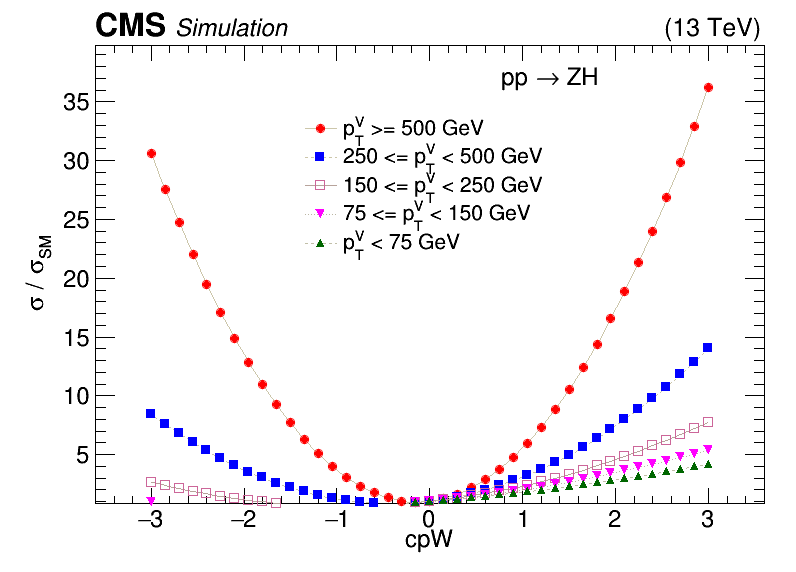
\includegraphics[width=0.321\textwidth]{Figures/LHE/ZH/Canv_cpW.png}
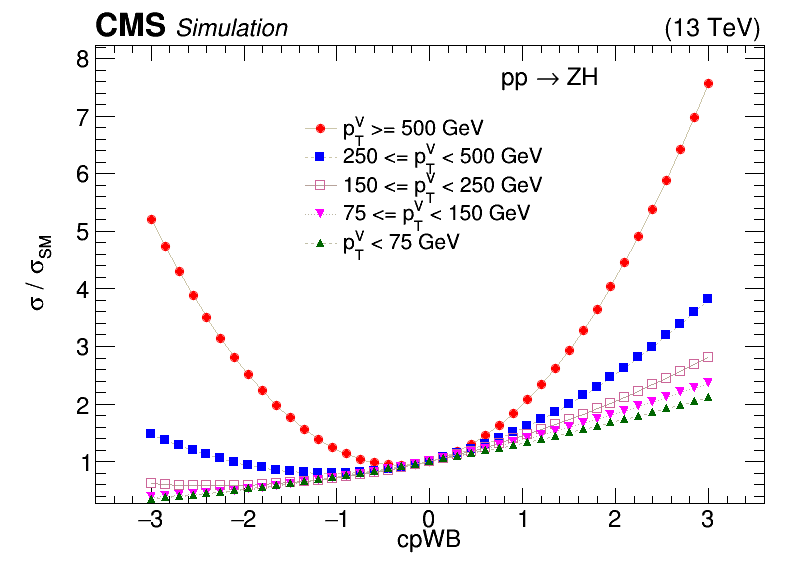
\includegraphics[width=0.321\textwidth]{Figures/LHE/ZH/Canv_cpWB.png}
\end{center}
\caption{
The ratio $\sigma/\sigma_{\textrm{SM}}$ of the cross section of the $\PW\PH$ (top) and $\PZ\PH$ (bottom) processes relative to the SM prediction as a function of Wilson coefficients ${\cal O}^{(3)}_{Hq}$ (left), ${\cal O}_{HW}$ (middle), and ${\cal O}_{HWB}$ (right) in five regions of $\PW$ and $\PZ$ boson {\pt}, respectively.
}
\label{fig:LHE_WZH}
\end{figure*}
The goal of this proposal is to probe the SM-EFT operators in Table~\ref{Tab:Operators}  as precisely as possible using events from the \VH processes in the data from the CMS experiment. 
The experimental work to excavate two distinct features, combined to achieve optimal sensitivity, are tackled separately.

In the first objective, I will exploit energy growth induced by 4-point SM-EFT interactions to boost the sensitivity of the differential cross section measurements in the leptonic \VH final states.
The three operators ${\cal O}^{(3)}_{Hq}$, ${\cal O}_{HW}$, their CP-odd counterparts, and the operators ${\cal O}_{HD}$, ${\cal O}_{H\square}$ affect both $\PW\PH$ and $\PZ\PH$ productions. 
I show the dependence of the production cross section on the first three Wilson coefficients for different selections of the in vector boson transverse momentum, $\pt(\PV)$, in Fig.~\ref{fig:LHE_WZH}. 
The energy growth is visible as an increased dependence on the Wilson coefficient for selections with higher $\pt(\PV)$. %FIXME <- Tell them what they see!
The operators ${\cal O}^{(1)}_{Hq}$, ${\cal O}_{Hu}$, ${\cal O}_{Hd}$, ${\cal O}_{HB}$, and ${\cal O}_{H\tilde{B}}$ affect only the $\PZ\PH$ production, 
because both left- and right-handed initial-state quarks of same flavor take part in $\PZ\PH$ production, while only the left-handed quarks of different flavors are involved in $\PW\PH$ production~\cite{Falkowski:2014tna,Banerjee:2018bio}. 
Therefore, measurements in both $\PW\PH$ and $\PZ\PH$ production are essential to probe the complete set of dimension-6 operators affecting $\PV\PH$ production.
%FIXME Can this be made more concrete? What helicity structure is responsible? --> Done
%Also, a reference is needed. --> Done
%What is the purpose of this statement? --> The answer lies in the last sentence of the last part in this section

In the second objective, I use a the angular observables to further boost the sensitivity and tackle the CP-structure of the \PV--\PH interaction. 
As an example, I show on of the angular variables, $\phi$, in Fig.~\ref{fig:LHE_phi}. 
Here, the leading contribution for the CP-even and -odd operators come the terms from corresponding to $f^{2}_{LT}$ and $\tilde{f}^2_{LT}$ in Eq.~\eqref{Eq:funcs}, respectively, which have $\cos\left(\varphi\right)$ and $\sin\left(\varphi\right)$ dependence.
%FIXME <- Here a link to the sinusodial variations is needed from Sec. 3. It should be stated that sin/cos is CP odd/even. Let's add a sentence when the table is there. --> Done
In the simpler $\PW\gamma$ final state, the technique increased the sensitivity by about a factor of 10~\cite{CMS-PAS-SMP-20-005}.
\begin{figure*}[hbtp]
\begin{center}
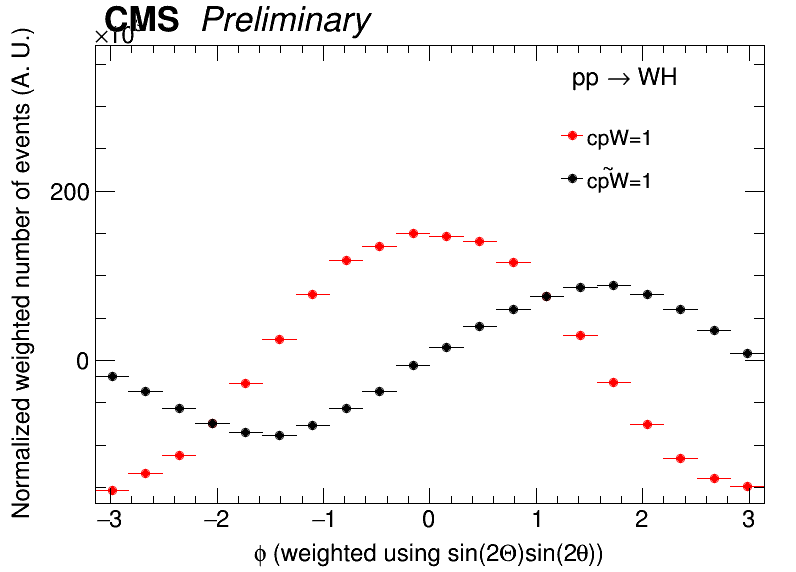
\includegraphics[width=0.45\textwidth]{Figures/LHE/WH/LHE_Plot_phi.png}
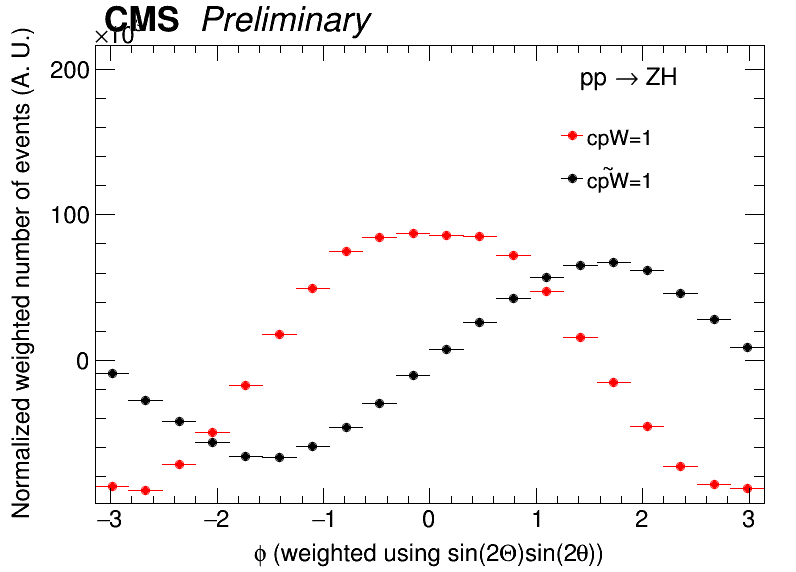
\includegraphics[width=0.45\textwidth]{Figures/LHE/ZH/LHE_Plot_phi.png}
\end{center}
\caption{
Distribution of angle $\phi$ for CP-even operator ${\cal O}_{HW}$  (red points) and CP-odd operator ${\cal O}_{H\tilde{W}}$ (black points) at the particle level in case of $\PW\PH$ (left) and $\PZ\PH$ (right) productions.
}
\label{fig:LHE_phi}
\end{figure*}

The SM cross section for $\PW\PH$ production with  $\PH\rightarrow\Pb\PAb$ and $\PW\rightarrow\ell\nu$  is 0.28 pb, whereas it is only 0.05 pb for $\PZ\PH$ production, where $\PZ\rightarrow\ell\ell$.
Thus, \PW process thus provides better statistical precision in the measurements. 
%FIXME Quote the x-sec numbers! --> Done
The \PZ final state is less populated but backgrounds are only at the X\% level, providing independent and corroborating evidence of the BSM signal. 
Therefore, simultaneous measurements of the couplings in both $\PW\PH$ and $\PZ\PH$ processes are necessary to confidently probe the complete set of operators relevant~\cite{Banerjee:2019twi}.
A preliminary sensitivity study is presented in Sec.~\ref{sec:method}. 

\section{Scientific originality}

%Although the SM-EFT operators can be indirectly probed using results from the previous experiments, 
The combined data sets from the LHC Runs 2 and the future LHC Run 3 provide an opportunity to measure SM-EFT operators involving the Higgs field~\cite{Elias-Miro:2013mua,Gupta:2014rxa} with unprecedented precision. 
In the $\PV\to\Pl\Pl$ and $\PH \to \Pb\PAb$ final state, I extend traditional search strategies, based on the basic STXS binning scheme~\cite{Berger:2019wnu}, by angular observables sensitive to subtle SM-EFT effects and the CP-structure of the \PV--\PH interaction. For the first time,

%So far, there exist very few measurements where all the efficiency and acceptance effects of object and event selection conditions are taken into account, and complete information contained in an event is used.
%The proposed measurement will extend the scope of probing new physics scenarios in the following ways.


\begin{itemize}

\item the complete multi-dimensional event information is used in \VH production to directly probe dimension-6 SM-EFT operators inducing energy growth.
Besides kinematic event properties, novel angular variables~(Fig.~\ref{fig:angles}) crucially refine the analysis strategy. 
They disentangling the various SM-EFT effects and can boost the sensitivity up to an order of magnitude~\cite{CMS-PAS-SMP-20-005}. Furthermore, 

\item the angular information, not explored previously in \VH production, is used to probe the CP structure of SM-EFT modifications of the \PV--\PH coupling. We can, therefore, measure new sources of CP violation beyond the SM.
\end{itemize}

Smaller novel items pertain to the multivariate~(MVA) analysis strategy employed to achieve these goals. 
%In the journey to achieve the goals, there will be possibilties to improve the techniques used in experimental measurements. 
For example, the proposer's group has recently developed a new technique to train tree-based classifiers to optimally separate effects of SM-EFT operators from the SM background~\cite{Chatterjee:2021nms}.
%Development of the methods and applying those in a CMS measurement by the same group will greatly accelerate the preparation of the results. 
%Also, efficiency of the deep neural network (DNN) based algorithms, used to identify \PH decaying to a pair of \Pb quarks, is conventionally measured in data and simulation in $\Pg \to \Pb \PAb$ process. 
%However, \Pg and \PH are very different in mass, spin, and color properties. During the proposed work, an effort will be pursued to improve the calibration of the tagger, 
%particularly using $\PZ \to \Pb \PAb$ decay.

\section{Relevance to the research field}

On a broad scale, the measurements provide a new piece of the TeV-scale SM-EFT puzzle. 
The findings will be interpreted in the context of SM-EFT which guarantees maximal independence from model assumptions and a smooth interface with theory interpretations.  

The absence of hints for resonant BSM phenomena has shifted the focus from ultraviolet-complete theories to EFTs, with first attempts at complete \TeV-scale characterizations emerging relatively recently~\cite{Ellis:2018gqa,Ellis:2020unq,Ethier:2021bye}.
At the experimental collaborations, the measurements of SM-EFT operator coefficients has arrived at the center stage of the LHC physics program~\cite{CMS:2021nnc,CMS:2021aly,CMS:2021gme}.
The interest from the theoretical and experimental communities is still growing, reflected in various new working groups (e.g. the  LHC EFT working group~\cite{LHC_EFT_WG}) and lecture series (e.g. ``All things EFT''~\cite{All_EFT}).

%The main relevance of the proposed research is to provide a novel building block for the characterization of BSM phenomena at the \TeV energy scale.


In particular, the proposed research contributes a unique probe of SM-EFT operator coefficients in the Higgs sector.
Besides the sensitivity boost from novel experimental techniques, it also complements the existing results by extending to CP-sensitive angular observables, tightly constraining the \PV--\PH couplings.
A deviation from the SM hinting at new sources of CP-violation will have wide-ranging significance in the explanation of the origin of the matter-antimatter asymmetry of the universe~\cite{Cohen:1997ac,Damgaard:2015con,Grzadkowski:2018nbc}.

%In particular, measurements of the vector couplings involving light quarks nicely complement the measurement of the similar couplings involving top quarks and they together can probe the flavor universality in quark sector in SM-EFT.

%Guided by, e.g., the effective description of beta decay in Fermi's theory~\cite{Fermi:1934hr} and Yukawa's theory of meson exchange~\cite{Yukawa:1935xg} EFTs ~\cite{Grinstein:1991cd,Alonso:2013hga,Brivio:2017vri,Passarino:2016pzb}  towards EFT as the future

The relevance of the proposed research extends to adjacent fields when the interplay of LHC measurements in global SM-EFT measurements is considered~\cite{Ellis:2018gqa,Ethier:2021bye}.
For example, specific assumptions of the BSM flavor structure provides a tight connection of the proposed measurement with the sector of top-quark physics. 
Moreover, the SM electroweak symmetry breaking relates the 4-point interactions in Table~\ref{Tab:Operators} to complementary measurements of the fermion-gauge boson couplings. 
An example of this link can be obtained from Fig.~\ref{fig:Feynman_digarams}~(left) when replacing the \PH boson line with the vacuum expectation value $v$.

The results obtained from the proposed measurements can also be reinterpreted as constraints on ultraviolet-complete new physics models describing the underlying dynamics at high energy.
Particular models the proposed analysis will be capable of probing are the following:
\begin{itemize}

\item Singlet scalar models, where a scalar field, singlet under the SM gauge group, is introduced~\cite{deBlas:2014mba,Profumo:2014opa}. This class of models gives rise to operators of the form of ${\cal O}_{H\square}$, ${\cal O}_{HD}$, ${\cal O}_{HW}$, ${\cal O}_{HB}$, ${\cal O}_{HWB}$, ${\cal O}_{Hu}$, and ${\cal O}_{Hd}$.

\item Models predicting the existence of a new vector boson~\cite{delAguila:2010mx}, for example, \PZprime and \PWprime. 
The models with extra spatial dimensions~\cite{Burdman:2006gy}, and little Higgs models~\cite{PhysRevD.10.275} fall in this category.
If the new bosons coupling to both fermions and gauge bosons has large mass ($>$ few \TeV), this gives rise to the contact interaction shown in Fig.~\ref{fig:Feynman_digarams} (left) and thus contributes to the operators  ${\cal O}^{(1)}_{Hq}$, ${\cal O}^{(3)}_{Hq}$, ${\cal O}_{Hu}$, and ${\cal O}_{Hd}$. 

\item Colored extensions of the SM with vector-like quarks (VLQs), triplet under SU(3) and singlet under SU(2)$_L$~\cite{delAguila:2000aa,Dawson:2012di}. 
When VLQs are allowed to couple to light quarks, they can give rise to ${\cal O}^{(1)}_{Hq}$ and ${\cal O}^{(3)}_{Hq}$ operators.
Particularly, new physics models with \PZprime or VLQs are in highlights in recent times to explain the anomalies in the flavor sector. 

\end{itemize}

The phenomenological implications of the \PV--\PH coupling measurement thus radiate into neighbouring research areas, while the proposed experimental program is self-contained.
In the following section, I aim to prove that. 

\section{Method}
\label{sec:method}

%Achieving goals in time requires setting up a concrete plan in advance. 
We target to utilize the combined data set from the LHC Run~2, corresponding to an integrated luminosity of 139\fbinv at $\sqrt{s}=13\TeV$, and the LHC Run~3, currently estimated at $\approx160\fbinv$.
With $45\%$ of the data available, we can develop and publish the novel analysis techniques during the third running period. 
When the full data set is available at the end of Run~3, we can obtain ultimate precision on a comparably short time scale and publish a benchmark result whose precision can not be surpassed until well into the HL-LHC research program.

In the following, we report the results of a feasibility study of the proposed measurements.
While the clean $\PZ\PH$ process serves as an independent search channel with orthogonal SM-EFT sensitivity, we focus on the more challenging $\PW\PH$ final states.
The results are equally valid for the $\PZ\PH$ case.

\subsection{Final states and observables}

In the SM, the $\PH \to \Pb \PAb$ decay channel has the largest branching ratio, motivating to choose it as a focus for improving  the statistical precision of the measurement.
Leptonic decay modes of the vector bosons help in reducing difficult backgrounds from the QCD multijet production.
In summary, we consider the $\PW\PH$ and $\PZ\PH$ production processes in the $\PW\to \Pl \Pgn$, $\PZ\to {\Pl}^{+} {\Pl}^{-}$, and $\PH \to \Pb \PAb $ decay channels, where $\ell=(\Pe, \Pmu)$.

%The following final states are considered.
%\begin{itemize}
%\item $\PW\left(\to \Pl \Pgn \right) \PH \left(\to \Pb \PAb %\right)$
%\item $\PZ\left(\to {\Pl}^{+} {\Pl}^{-} \right) \PH \left(\to \Pb \PAb \right)$
%\end{itemize}


As shown in Sec.~\ref{sec:objective} and Fig.~\ref{fig:LHE_WZH}, the 4-point interactions provided by the operators in Table.~\ref{Tab:Operators} induce  energy growth, modifying the highly energetic tail of distributions of kinematic observables such as the transverse boson momenta, $\pt(\PW)$, $\pt(\PZ)$, or $\pt(\PH)$. 
These kinematic observables are not sufficient to disentangle the various effects from the large number of possible SM-EFT operators. 
A systematic analysis of helicity amplitudes in \VH production decay is provided in Ref.~\cite{Banerjee:2019twi}. 
Amplitudes involving the longitudinal and transverse vector boson polarizations contribute differently to \VH production, in both the SM and in SM-EFT. 
The interference among helicity amplitudes, including CP effects, is preserved at the event level in subtle angular triple-correlations. 
%FIXME Specify when table is there. --> Done
For example, the cosinusoidal and sinusoidal modulations in $\phi$ distributions shown in Fig.~\ref{fig:LHE_phi} are obtained after using the sign of $\sin\left(2\Theta\right)\sin\left(2\theta\right)$ as seen from $\tilde{f}^2_{LT}$ and $f^2_{LT}$ terms, respectively in  Eq.~\ref{Eq:funcs}. 
This allows to extract rich information about the event structure from a joint analysis of kinematic and angular variables.

Specifically, Ref.~\cite{Banerjee:2019twi} proposes to reconstruct the novel angular variables shown in Fig.~\ref{fig:HelicityFrame}. 
It is important to note that traditional strategies can not leverage the subtle angular triple-correlation: integrating any of the angles in the final observables removes the interference effects~\cite{Panico:2017frx}.


\begin{comment}
once calculates helicity amplitudes in \VH center-of-mass frame and the cross section has the following form:
\begin{equation}
{\sigma}_{\VH} (\hat{s},\Theta,\theta,\phi) = {\sum}_{i=1}^{9} a_{i}(\hat{s}) f_{i}(\Theta,\theta,\phi)	\ .
\label{Eq:Xsection}
 \end{equation}  
In Eq.~\eqref{Eq:Xsection}, $a_{i}$, parameterizing the dependence of Wilson coefficient and energy transfer $\hat{s}$, are known as angular moments and $f_{i}$ encapsulates the dependency on the angles $\Theta,\theta,\phi$ defined in Fig.~\ref{fig:HelicityFrame}.
\begin{figure*}[hbtp]
\begin{center}
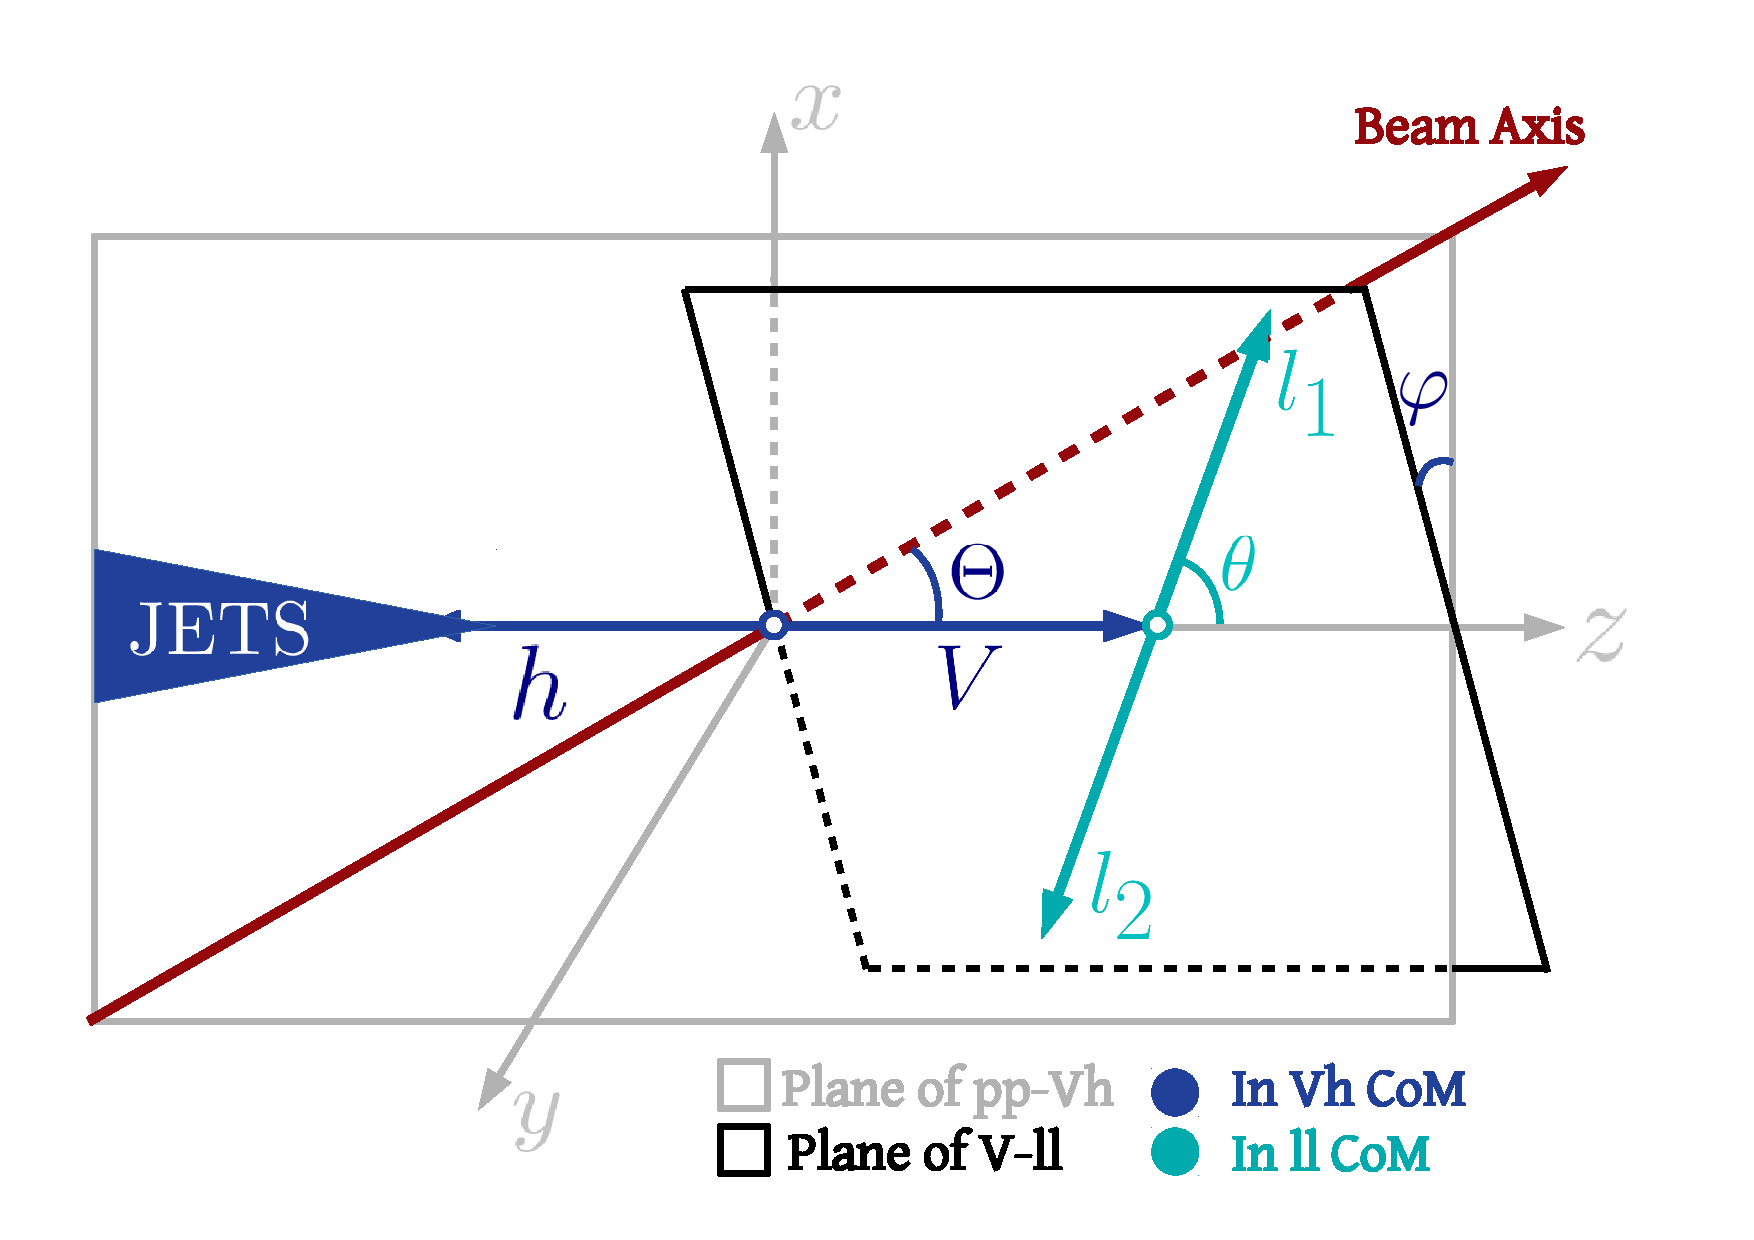
\includegraphics[width=0.75\textwidth]{Figures/LHE/TheThreeAnglesVh.pdf}
\end{center}
\caption{
Definition
}
\label{fig:HelicityFrame}
\end{figure*}
The functions $a$ and $f$ contain the complete information of how \VH production is affected by dimension-6 SM-EFT operators and their forms can be found in Ref.~\cite{Banerjee:2019twi}. 
However, the absence of knowledge about the directions of incoming quark and anti-quark leads to the vanishing of three angular moments. Among the remaining six angular moments, two correspond to the case where the vector boson is either transversely or longitudinally polarized, and the remaining four correspond to the interference of two amplitudes with different polarizations of the vector boson. An inclusive measurement over all the angles lead to the vanishing of the later four angular moments, thus a loss of information about the event structure. 

In this proposal, we target to use complementary kinematic and angular observables in \VH process and probe the SM-EFT operators at work.


We consider the final states as follows.
\begin{itemize}
\item $\PW\left(\to \Pl \Pgn \right) \PH \left(\to \Pb \PAb \right)$
\item $\PZ\left(\to \Pl \Pl \right) \PH \left(\to \Pb \PAb \right)$
\end{itemize}
Since $\PH \to \Pb \PAb$ has the largest branching ratio, its use enables to improves the statistics of the analyzed event sample. 
Leptonic decay of the vector boson helps to get rid of the background from the multijet production in QCD, which is the dominant background in most of the hadronic final states. 
The lepton(s) from the vector boson also helps to trigger the events. The process $\PZ\left(\to \Pgn \Pgn \right) \PH \left(\to \Pb \PAb \right)$ is ignored here since we need the lepton directions to construct the angular variables.
\end{comment}

\subsection{Event selection and categorization}

The CMS trigger system selects the \VH events based in the presence of leptons~(electrons or muons) originating from the \PW or \PZ bosons. 
At moderate momenta, single- and double lepton triggers are used.
%The trigger system, developed centrally within the CMS Collaboration, is used to select events with at least one lepton (\Pl) satisfying a threshold in {\pt}.
At high $\pt(\PV)$, backup trigger paths requiring considerable hadronic activity are used to recover
efficiency losses for events with highly asymmetrical $\PV$ decay or with a highly energetic electron. 

The measurement of the trigger selection efficiency ratio between data and simulation is a standard (but important) step towards reducing the total systematic uncertainty.
For this purpose, we use tag-and-probe methods with $\PZ \to {\Pl}^{+} {\Pl}^{-}$ events to obtain event-level corrections factors that scale the simulation to the data . 
For the remainder of the feasibility study, we assume that simulation correctly predicts the trigger selection efficiency. 
All results are obtained from events simulated with \texttt{Madgraph5\_aMC@NLO}~\cite{Alwall:2014hca} and simulated up to the CMS detector level. 
The SM-EFT effects are incorporated with \texttt{MadWeight}~\cite{Artoisenet:2008zz} and using the \texttt{SMEFTsim}~model~\cite{Brivio:2017btx}.

After the trigger decision, we select $\PW\PH$ candidate events by requiring an electron or a muon with \pt$>32$ and $>25$\GeV, respectively. 
The CMS identification lepton criteria in the Run 2 data set correspond to 90 and 95\% efficiency for genuine electrons and muons, respectively. 
As will be discussed in Sec.~\ref{sec:neu_reco}, the four-momentum of the neutrino from the $\PW$ decay is reconstructed using the missing transverse momentum vector (\ptvecmiss), assuming that the invariant mass of neutrino-lepton system equals $m_{\PW}$ 
%This will be discussed further in . 

A sample enriched in boosted \PW bosons is selected by the requirement $\pt(\PW) > 150$\GeV. 
After this selection, the level of QCD multijet production is negligible.
Requiring a minimum difference of the azimuthal lepton- and \ptmiss angles, $\Delta\phi(\ell,\ptvecmiss)>2$, removes events with spurious signals while retaining good signal efficiency.
Finally, \PW candidate events must not to contain additional electrons or muons with $\pt>25$\GeV.

The selected events are further categorized into measurement regions depending on quantities from the jet system. 
If the \PH boson has large \pt, its decay products are merged into a jet with large cone size. 
In this ``boosted topology'', the \PH boson is reconstructed and identified in a the set of jets provided by the anti-\kt algorithm with distance parameter of $R=0.8$~(AK8 jets).
Otherwise, the \PH boson is in the ``resolved topology'' where it can be reconstructed using standard AK$4$ jets originating from the \Pb quark pair. 
In the boosted topology, the deep neural network~(DNN) based taggers DeepJet~\cite{Bols:2020bkb} and DeepAK8~\cite{Sirunyan:2020lcu} are used to identify AK4 subjets in the AK8 jet that correspond to the \Pb quark pair.
The DeepAK8 tagger provides probability-normalized classifier values for the top quark, \PW boson, light quark or gluon hypothesis for each AK8 jet. We use this information later on for signal-to-background discrimination in the boosted topology. % FIXME Be specific --> Done

In the resolved topology, the two AK4 jets with highest \Pb tagging scores, referred to as $\textrm{b}_{1(,2)}$, form the \PH candidate, while the AK8 jet ($\textrm{J}$) with the highest \PH tagging score provides the \PH candidate in the boosted topology.
Fot AK8 jets, soft drop grooming~\cite{Larkoski:2014wba} is used to calculate the mass by removing the uncorrelated radidation clustered into the jet. 
The signal region (SR), enriched by $\PW\left(\to \Pl \Pgn \right) \PH \left(\to \Pb \PAb \right)$ events, is constructed using the conditions listed in Table~\ref{Tab:Regions}.

{\renewcommand{\arraystretch}{1.3}
\begin{table}[t]
\centering
\caption{
Selection conditions targeted for $\PW\PH$ events.
}
\begin{tabular}{p{60mm}|p{60mm}}
%\begin{tabular}{lcl |lcl}
Resolved category & Boosted category \\
\hline
%Two AK4 jets with highest \Pbottom tagging score (say, b1, b2) & AK8 jet with the highest \PHiggs tagging score \\
At least 2 b-tagged AK$4$ jets \newline (satisfying $\pt>30\GeV$, $|\eta|<2.5$)  & At least 1 AK8 jets \newline (satisfying $\pt>250\GeV$, $|\eta|<2.5$) \\
The {\Pb} tagging score of  $\textrm{b}_1>$ btag$^{\text{cut}}_{\text{max}}$ & The \PH tagging score of \PH $>$ Htag$^{\text{cut}}$\\
The {\Pb} tagging score of $\textrm{b}_2>$ btag$^{\text{cut}}_{\text{min}}$ & \\
Up to 1 additional AK4 jets & Veto on extra b-tagged AK4 jets  \\%FIXME: Really "<" ? --> Yes
%$90<M(\textrm{b}_1,\textrm{b}_2)<150~\GeV$ & $90<M_\textrm{SD}<150$~\GeV \\
$M(\textrm{b}_1 + \textrm{b}_2) \in \left[90, 150\right]~\GeV$ & Soft-drop mass of $\textrm{J} \in \left[90, 150\right]~\GeV$ \\
\end{tabular}
\label{Tab:Regions}
\end{table}
}
In Table~\ref{Tab:Regions}, the threshold values btag$^{\text{cut}}_{\text{max}}$ and btag$^{\text{cut}}_{\text{min}}$ are chosen to ensure a DeepJet b-tagging mistag rate of 1\% and 10\%  for light quark or gluon jets, respectively.
The threshold value Htag$^{\text{cut}}$ corresponds to a \PH mistag rate of 1\%.

Inverting specific requirements in  Table~\ref{Tab:Regions}, defines control regions (CRs), enriched by the various background processes. 
For example, requiring two or more AK4 jets  in the resolved category or the presence of b-tagged AK4 jets in the boosted category selects an event sample enriched with top quark pair production ($\Pt\PAt$).
Inverting the mass window on the \PH candidate results in a CR dominated by vector boson production in association with $\Pb$- and $\Pc$-quark jets (${\PW}+\Pb/\Pc$). 
Finally, resolved~(boosted) events failing the the requirement of the presence of two b-tagged AK4 jets (one Higgs-tagged AK8 jet) are dominated by vector boson production in association with light quark or gluon jets (${\PW}+$udsg).
These CRs are used to measure and validate the corresponding backgrounds in data.

The distribution of $\pt(\PW)$ in the resolved and boosted SR are shown in Fig.~\ref{fig:RECO_Vpt_WH}, where alternate $\PW\PH$ signal hypothesis for the operators ${\cal O}^{(3)}_{Hq}$ and ${\cal O}_{HW}$  are overlaid. 
\begin{figure*}[hbtp]
\begin{center}
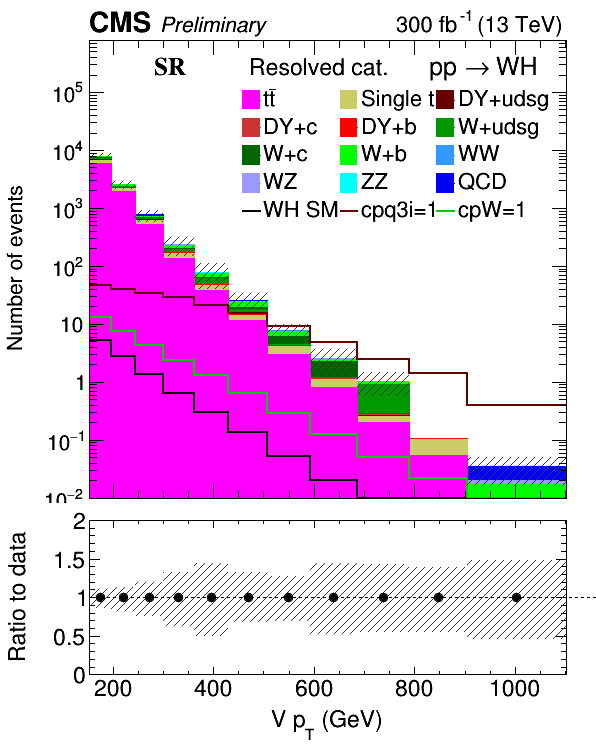
\includegraphics[width=0.475\textwidth]{Figures/RECO/Plot_Resolved_SR_V_pt.png}
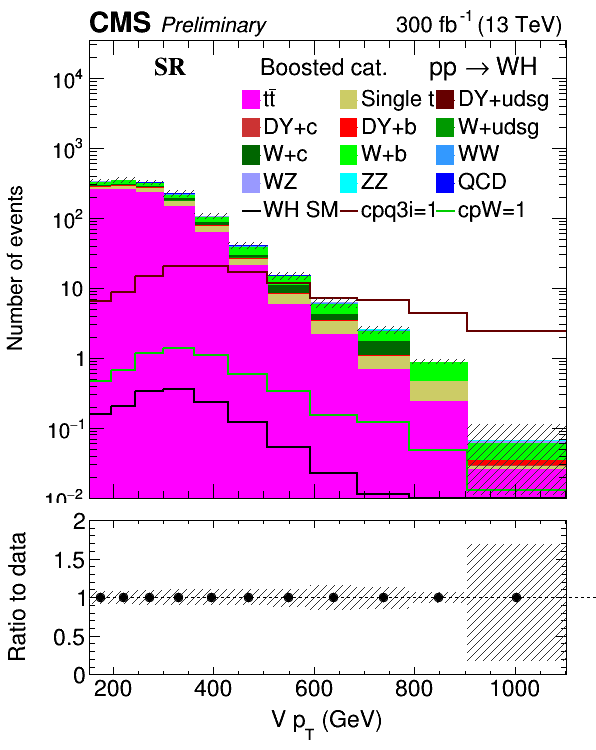
\includegraphics[width=0.475\textwidth]{Figures/RECO/Plot_Boosted_SR_V_pt.png}
\end{center}
\caption{
Distribution of \PW boson \pt in the resolved (left) and boosted (left) categories of the SR. Impact of systematic uncertainties on jet energy scale and resolution, correction factor used to match the b-tagging and Higgs-tagging efficiencies in data and simulation are shown in the bottom panel.
}
\label{fig:RECO_Vpt_WH}
\end{figure*}
The figure shows the importance of the $\Pt\PAt$, ${\PW}+\Pb/\Pc$, and ${\PW}+\textrm{udsg}$ backgrounds in the  $\PW\PH$ SRs.

Next we turn to the sensitivity of the angular observables. As shown in Fig.~\ref{fig:angles}, 
the SM production, dominated by longitudinal polarization of \PW boson, exhibits differences in $\Theta$ for nonzero ${\cal O}_{HW}$  coefficients, because this operator  enhances the helicity amplitude of \PV\PH production with transverse polarizations.%FIXME Please check the correctness. --> Done
The observable $\phi$, on the other hand, is very sensitive to the CP-nature of the \PV--\PH coupling, and the difference in modulation of CP-even and CP-odd operator coefficients is clearly visible.  
The CP-sensitivity in the $\phi$ observable is slightly affected by the ambiguities introduced by the unknown $z$ momentum of the neutrino entering the $\PW$ momentum reconstruction. 
This necessiates to develop a sophisticated algorithm for neutrino reconstruction, possibly similar to the MVA-based technique designed in top quark analyses for assigning reconstructed objects to particles produced in the hard interaction~\cite{CMS:2019esx}.
%FIXME Suggest to motivate a selection MVA for the neutrino momentum as we do in tW reco ... adds an action item --> Done
The $\phi$ observable is weighted by $\sin2\Theta\sin2\theta$ to lift the cancellation otherwise enforced by the triple angular correlation. 
For the first time, we thus resurrect the interference of the helicity amplitude in \PH final states at the detector level. 
Comparing these predictions to the Run 2 and 3 data from the CMS experiment is a central goal of the proposal.

\begin{figure*}[hbtp]
\begin{center}
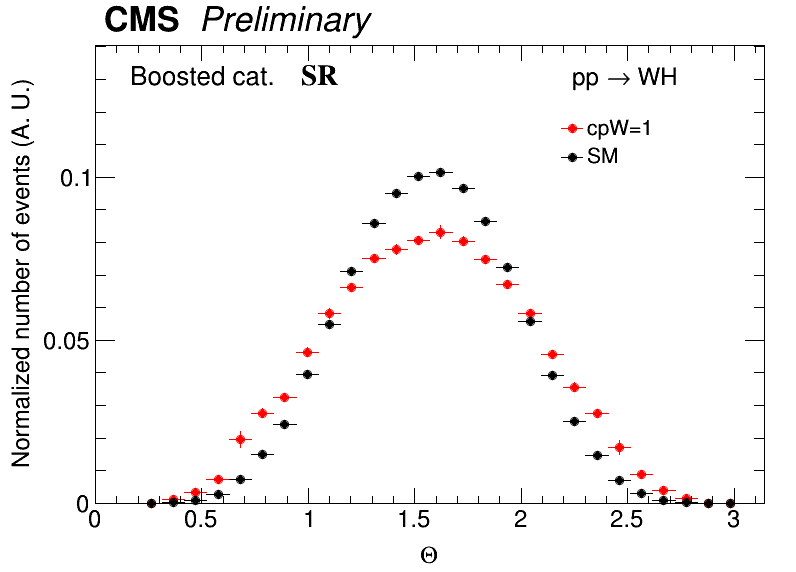
\includegraphics[width=0.475\textwidth]{Figures/RECO/Angle/WH/Boosted_Plot_Theta.png}
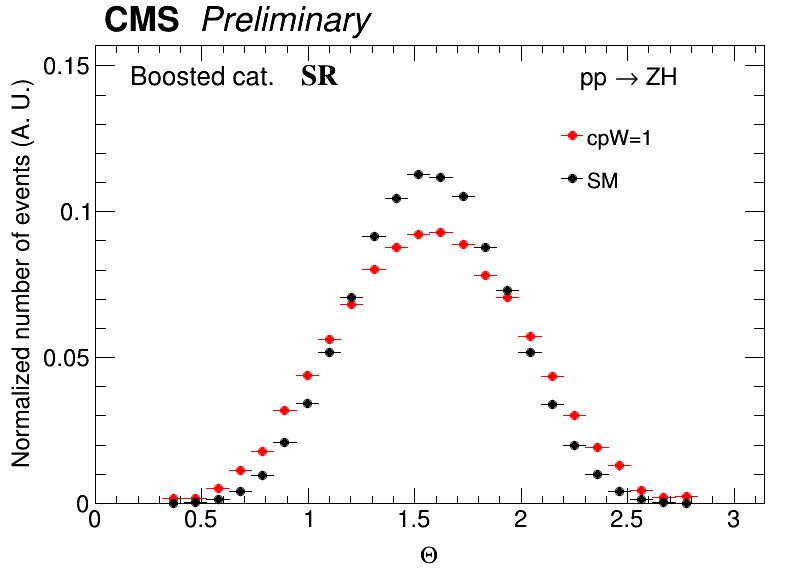
\includegraphics[width=0.475\textwidth]{Figures/RECO/Angle/ZH/Boosted_Plot_Theta.png}
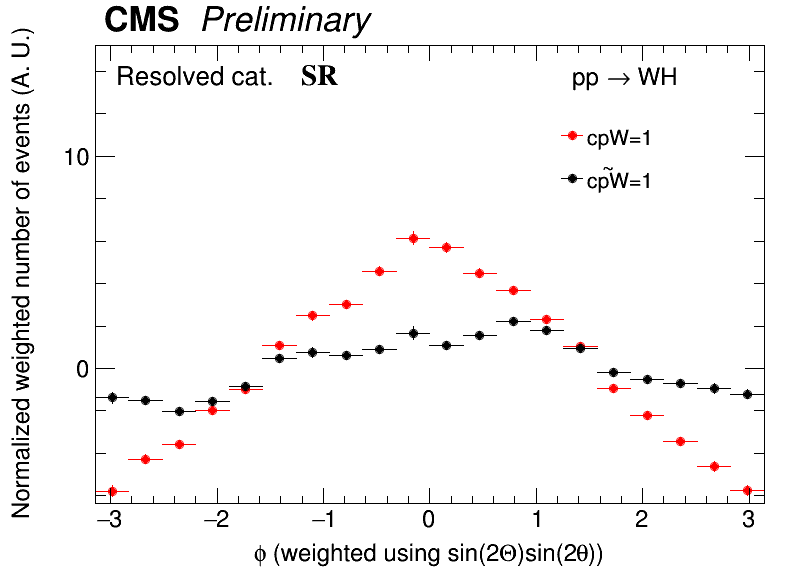
\includegraphics[width=0.475\textwidth]{Figures/RECO/CP/WH/Resolved_Plot_phi.png}
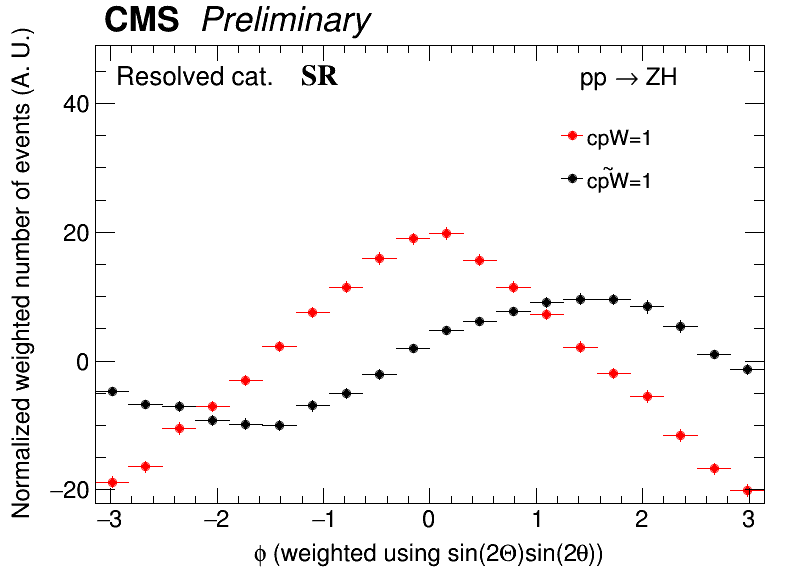
\includegraphics[width=0.475\textwidth]{Figures/RECO/CP/ZH/Resolved_Plot_phi.png}
\end{center}
\caption{
Normalized distribution of polar angle $\Theta$ in $\PW\PH$ (top left) and $\PZ\PH$ (top right) productions for $cpW=1$ and SM scenarios in the boosted category. 
Normalized distribution of azimuthal angle $\phi$ in  $\PW\PH$ (bottom left) and $\PZ\PH$ (bottom right) productions for $cpW=1$ and $\tilde{cpW}=1$, respectively; SM component is subtracted from in these distributions.
}
\label{fig:angles}
\end{figure*}

\subsection{Neutrino reconstruction}
\label{sec:neu_reco}

In order to reconstruct the momentum of invisible neutrino in $\PW \to \Pl \Pgn$, we assume that the \Pnu is the only source of $\ptvecmiss$ in the event and take its $\pt$ and $\phi$ as the same of \Pnu. 
In a simple approach, we use the quadratic equation from the $\PW$-mass constraint to calculate $\eta(\Pnu)$. 
The two possible solutions are
\begin{eqnarray}
\eta(\Pnu) &=& {\eta}(l) \pm \cosh^{-1}(1+{\Delta}^2),\;\textrm{where}\label{Eq:NeuEta}\\
{\Delta}^2 &=& \frac{m_W^2 - m_\textrm{T}^2 (\ell,{p^\text{miss}\xspace})}{2 p_\textrm{T}^{l}\, p_\textrm{T}^\textrm{miss}}. 
\end{eqnarray}
Large $\pt(\PW)$ leads to $\Delta \ll 1$, and the two solutions become 
\begin{equation}
{\eta}(\Pnu) \simeq {\eta}(\ell) \pm \sqrt{2}{\Delta} + {\cal{O}} ({\Delta}^3)	\ .
\label{Eq:NeuEta2}
\end{equation}
In this limit,  the angular variable $\theta$ and $\Theta$ converge to the same values, whereas a two-fold ambiguity  $\phi_{+} \simeq \pi - \phi_{-}$ remains for $\phi$. 
\begin{figure*}[hbtp]
\begin{center}
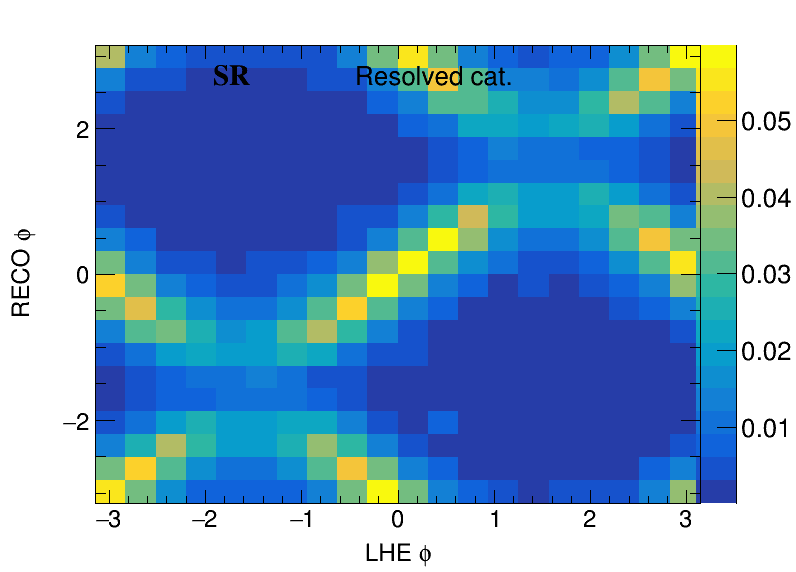
\includegraphics[width=0.495\textwidth]{Figures/RECO/Resolved_Plot_2D_phi_unweighted.png}
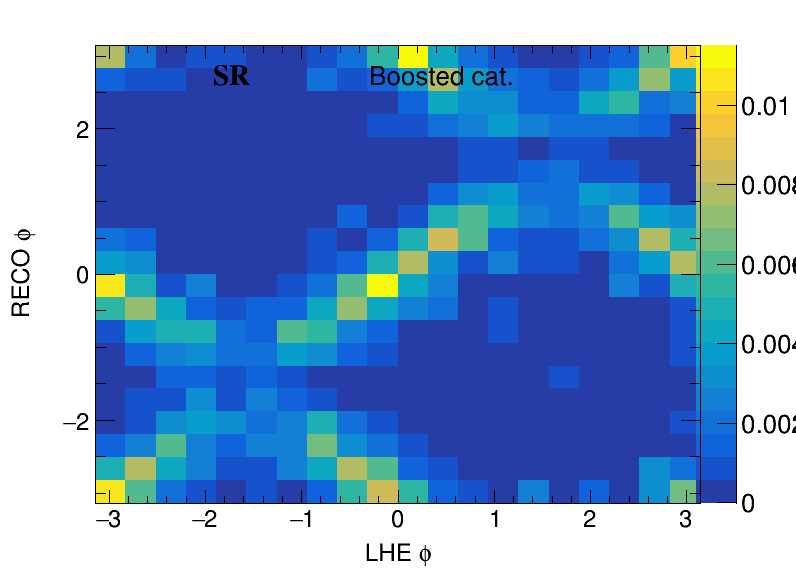
\includegraphics[width=0.495\textwidth]{Figures/RECO/Boosted_Plot_2D_phi_unweighted.png}
\end{center}
\caption{
Correlation between $\phi$ calculated at parton level and detector level in the resolved (left) and boosted (right) categories in $\PW\PH$ production.
}
\label{fig:neureco}
\end{figure*}
This ambiguity is visible in Fig.~\ref{fig:neureco} and currently reduces the CP-sensitivity in $\PW\PH$ production. 
No attempt was made to reduce the impact of the ambiguity for the purpose of this proposal. 
As part of the analysis development, we will develop a multi-variate discriminator to select the correct solution based on the kinematic event properties. %FIXME Add a reference to a successful strategy. --> Added in earlier section

\subsection{Multivariate analysis}

As shown in Fig.~\ref{fig:RECO_Vpt_WH}, the SRs are subject to significant backgrounds from top quark pair  and vector boson production.
To separate the  $\PW\PH$ and $\PZ\PH$ signals optimally from the backgrounds, MVA discriminators are constructed. 
In this study, it comprises two fully connected dense layers, while the discriminator will be promoted to an DNN in the analysis with real data.
A very preliminary set of input variables is listed in Table~\ref{Table:MVA_Vars}.
Variables in two columns in the upper group are used for the extraction of $\PW\PH$ and $\PZ\PH$ signals, respectively.
Left and right columns in the lower group list variables characterizing the jet system in the resolved and boosted categories, respectively, for the separation of both $\PW\PH$ and $\PZ\PH$ signals.
{\renewcommand{\arraystretch}{1.3}
\begin{table}[t]
\centering
\caption{
Input variables to the MVA discriminator designed to separate events from $\textrm{\PV}\PH$ and $\Pt\PAt$ productions.}
\subcaption*{Lepton-specific variables for $\PW\PH$ (left) and $\PZ\PH$ (right) signals.}
\begin{tabular}{l l}
\pt component of \ptvecmiss &  \pt and $\eta$ of the leading lepton\\
\pt and $\eta$ of the lepton & \pt and $\eta$ of the subleading lepton \\
$\Delta\phi(\Pl,\ptvecmiss)$ & $\Delta\phi({\Pl}_1,{\Pl}_2)$ \\
$\Delta\phi(\PW,\PH)$ & $\Delta\phi(\PZ,\PH)$ \\
Event thrust (see definition in~\cite{CMS:2014tkl}) & Event thrust\\
\end{tabular}
\bigskip
\subcaption*{Variables characterizing the jet system in resolved (left) and boosted (right) categories.}
\begin{tabular}{l l}
B-tagging scores of $\textrm{b}_1$ and $\textrm{b}_2$ & DeepAK8 top tagging score \\
$\textrm{Min}(\pt(\textrm{b}_1), \pt(\textrm{b}_2))$ and $\textrm{b}_2$ & DeepAK8 \PW tagging score \\
$\textrm{Max}(\pt(\textrm{b}_1), \pt(\textrm{b}_2))$ & DeepAK8 \Pb\PAb tagging score \\ 
$\textrm{Max}(\pt(\textrm{b}_1)/\pt(\ell), \pt(\textrm{b}_2)/\pt(\ell))$ & Rapidity and mass of \PH candidate \\
$\Delta\phi(\text{b}_1,\text{b}_2)$ & \\
Rapidity and mass of \PH candidate & \\
AK4 jet multiplicity \\ (satisfying $\pt>30\GeV$, $|\eta|<2.5$)  & \\
\end{tabular}
\label{Table:MVA_Vars}
\end{table}
}
%FIXME Add the following variables to the table. Add also a columns for ZH. --> Done
%A similar discriminator is built in the boosted category using the variables in the left column of Table~\ref{Table:MVA_Vars} along with the following variables corresponding to the \PH candidate AK8 jet: 
%the output of DeepAK8 taggers quantifying the probability of the jet originated due to top quark, Higgs boson, \PW boson relative to the same originated from a light quark or gluon.
Normalized distributions of MVA discriminators in SM $\PW\PH$ and $\Pt\PAt$ events are shown in Fig.~\ref{fig:MVA}. 
\begin{figure*}[hbtp]
\begin{center}
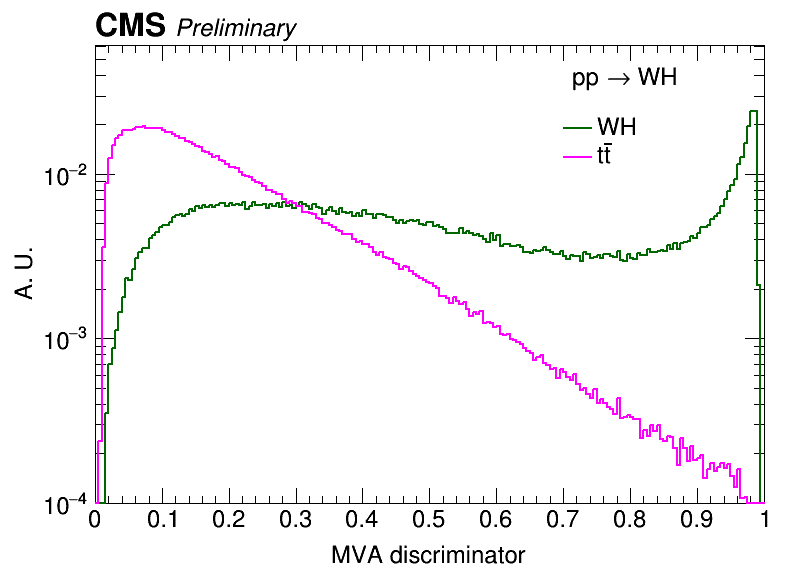
\includegraphics[width=0.475\textwidth]{Figures/RECO/Plot_WH_MVA_WH_fast_resolved.png}
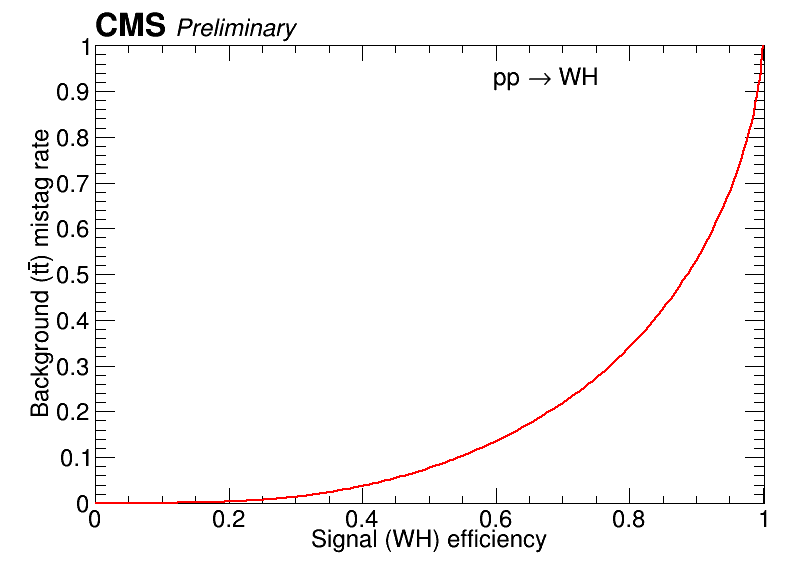
\includegraphics[width=0.475\textwidth]{Figures/RECO/ROC_plot_TT_MVA_resolved.png}
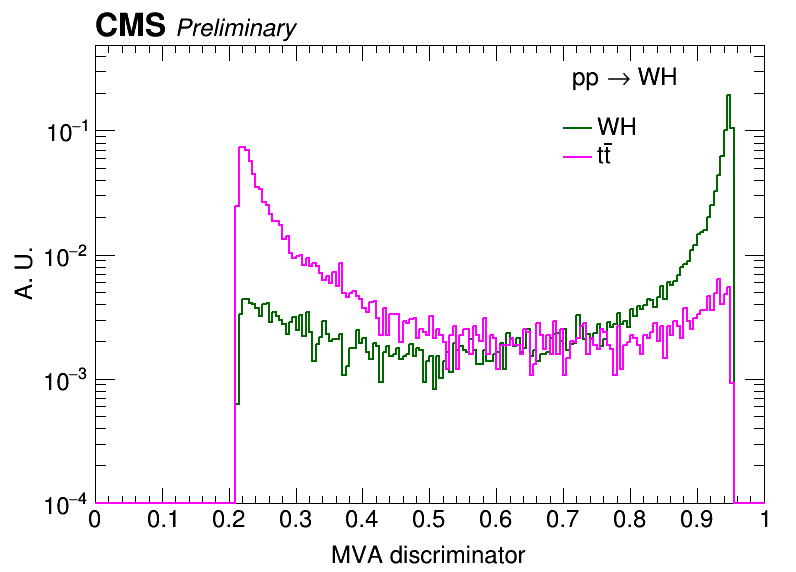
\includegraphics[width=0.475\textwidth]{Figures/RECO/Plot_WH_MVA_WH_fast_boosted.png}
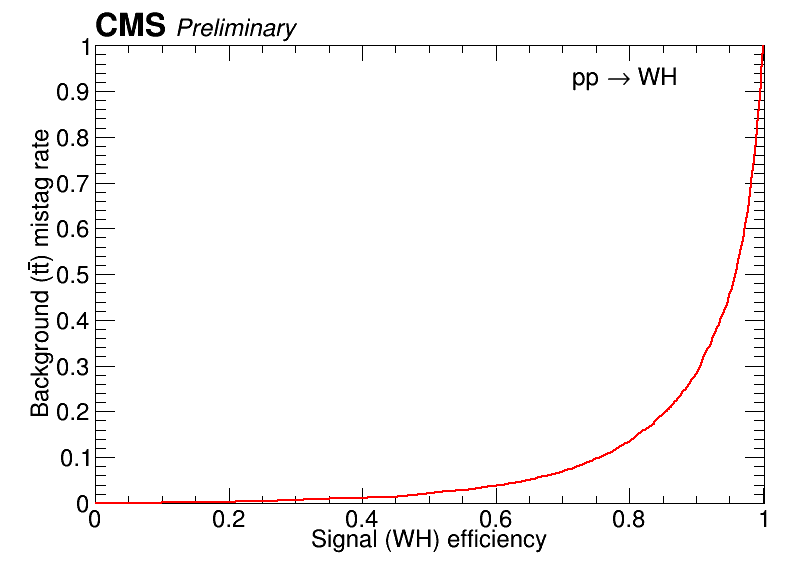
\includegraphics[width=0.475\textwidth]{Figures/RECO/ROC_plot_TT_MVA_boosted.png}
\end{center}
\caption{
Normalized distributions of the MVA discriminator in signal ($\PW\PH$) and background ($\Pt\PAt$) events (left) and ROC curve characterizing the performance of MVA discriminator (right) in the resolved (top) and boosted (bottom) categories.
}
\label{fig:MVA}
\end{figure*}
The output discriminator shapes and the performance of the discriminator, quantified with ROC curves~\cite{FAWCETT2006861}, are shown in Fig.~\ref{fig:MVA}. 
Benefiting from the DeepAK8 tagger outputs, the discriminator constructed in the boosted category performs slightly better. In both cases, the signal distribution is sharply peaked at high discriminator values, indicating a successfully trained classifier.
In the next section, we quantify the sensitivity gain from this strategy.

\subsection{Sensitivity results}

Although the final condition on the MVA discriminator are subject to development during the project, 
we can obtain a simple assessment of the sensitivity with a threshold on the MVA discriminator corresponding to a signal efficiency of $80\%$ signal.
This choice corresponds to a background efficiency of $\sim 30\%$ ($\sim 15\%$) in the resolved (boosted) category.
Next, we perform one-dimensional likelihood scans for the two Wilson coefficients corresponding to the operators ${\cal O}^{(3)}_{Hq}$ and ${\cal O}_{HW}$, respectively, while setting all other Wilson coefficients to $0$. 
Normalizing the predicted yields to an integrated luminosity of 300\fbinv, we show the negative log-likelihood results in in Fig.~\ref{fig:NLL}. %FIXME Define q, is it profiled? --> Done
\begin{figure*}[hbtp]
\begin{center}
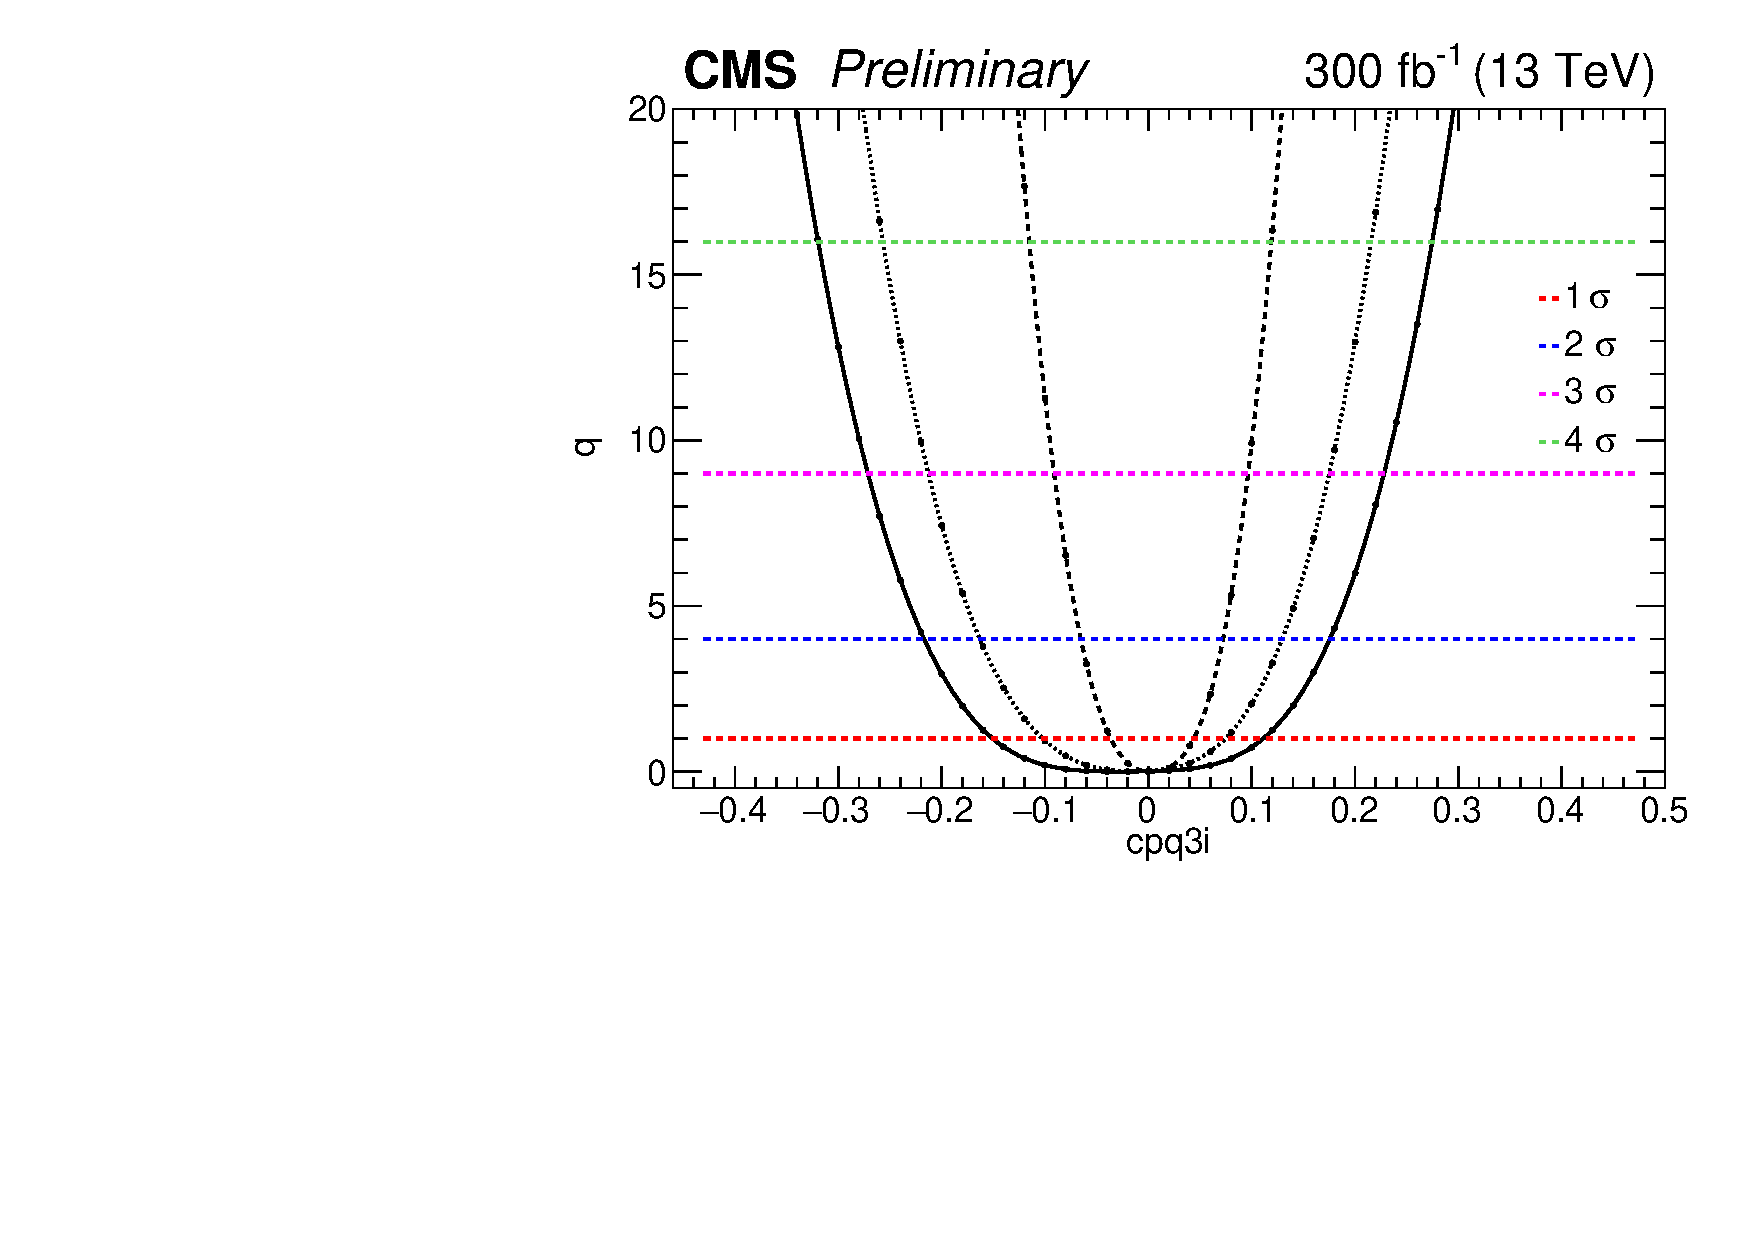
\includegraphics[width=0.495\textwidth]{Figures/RECO/Full_NLL_WC_cpq3i_fine_2019_opt2.pdf}
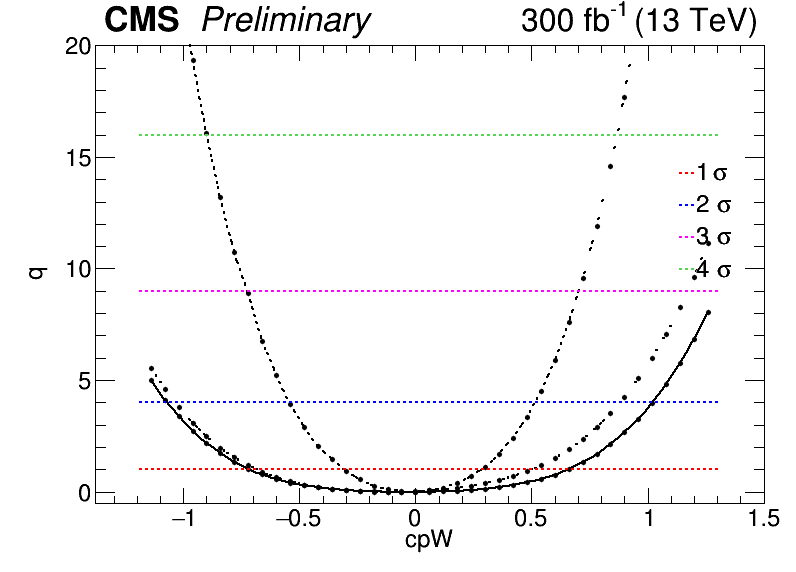
\includegraphics[width=0.495\textwidth]{Figures/RECO/Full_NLL_WC_cpW_fine_2019_opt2.png}
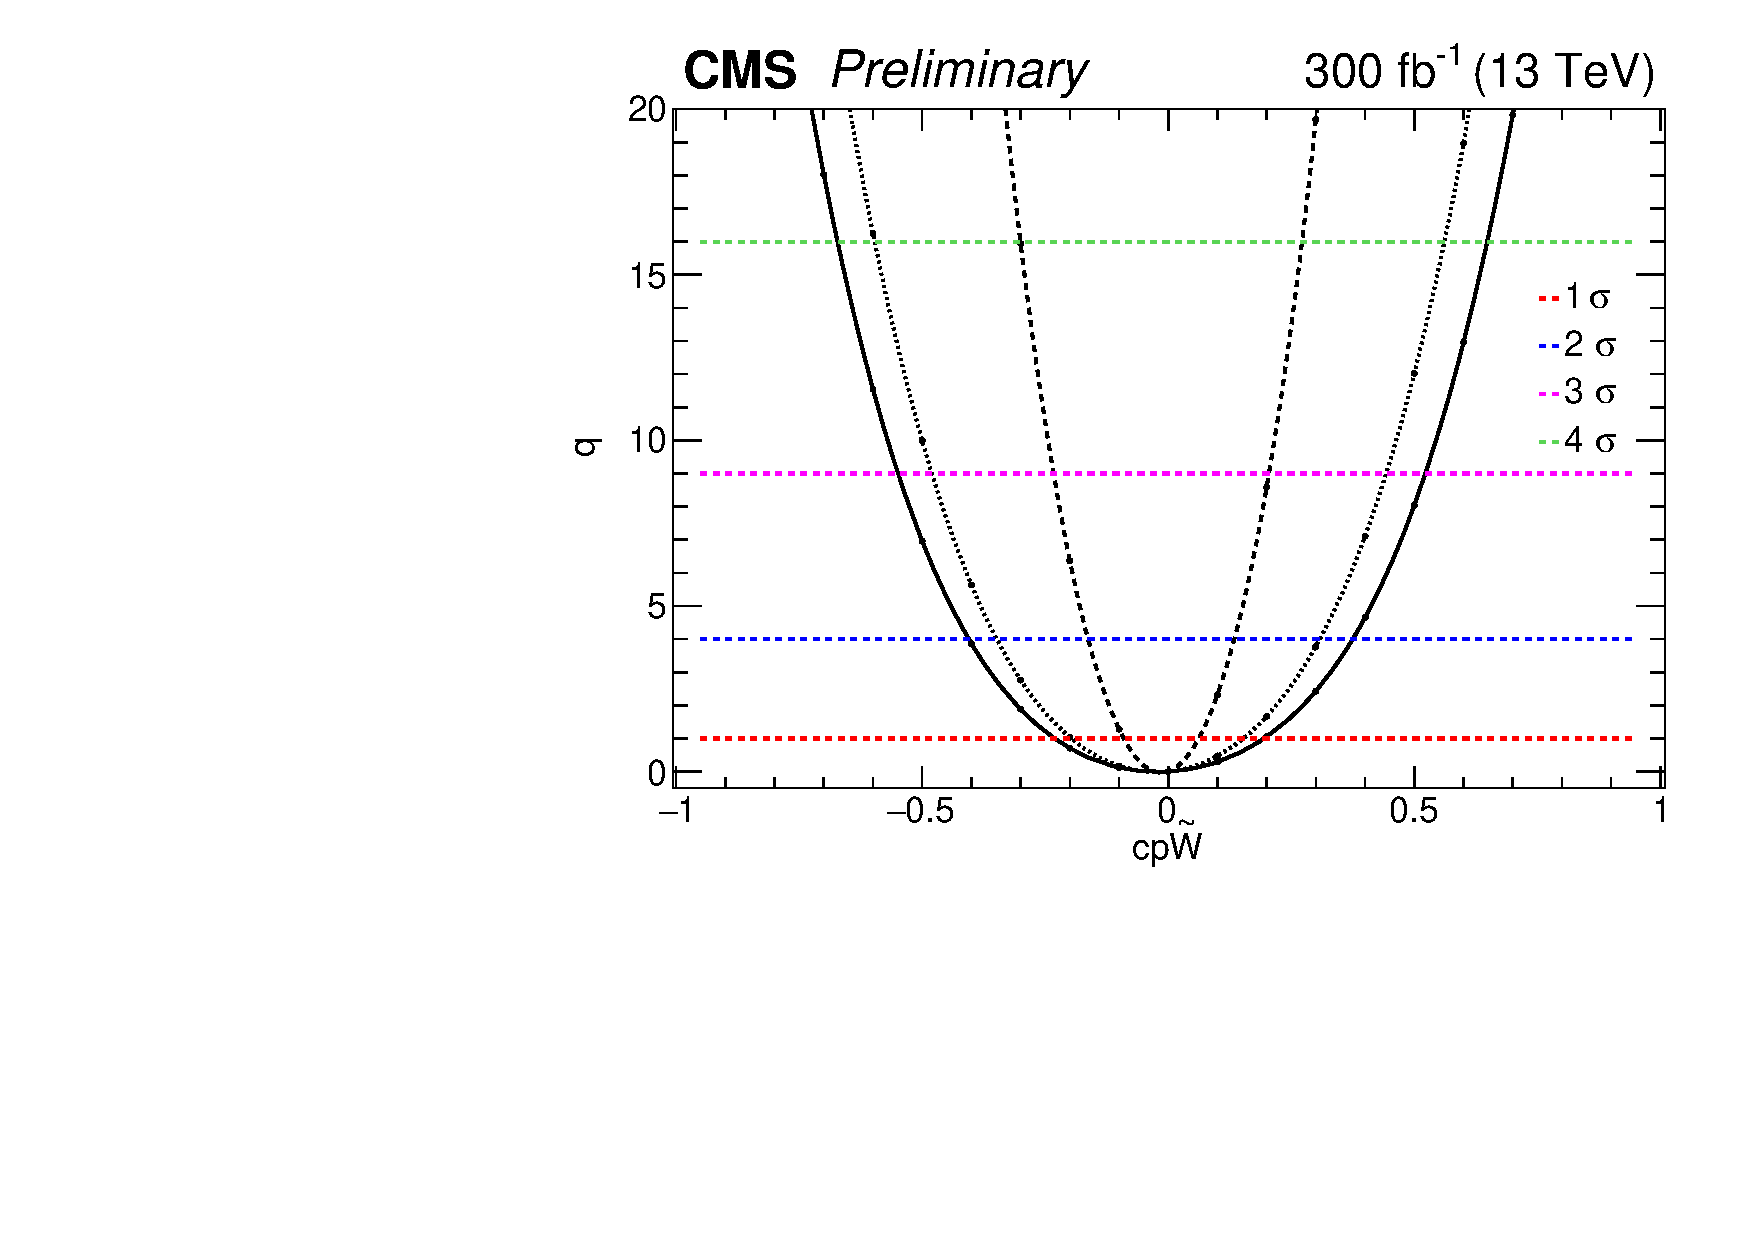
\includegraphics[width=0.495\textwidth]{Figures/RECO/Full_NLL_WC_cpWtilde_2019_opt2.pdf}  
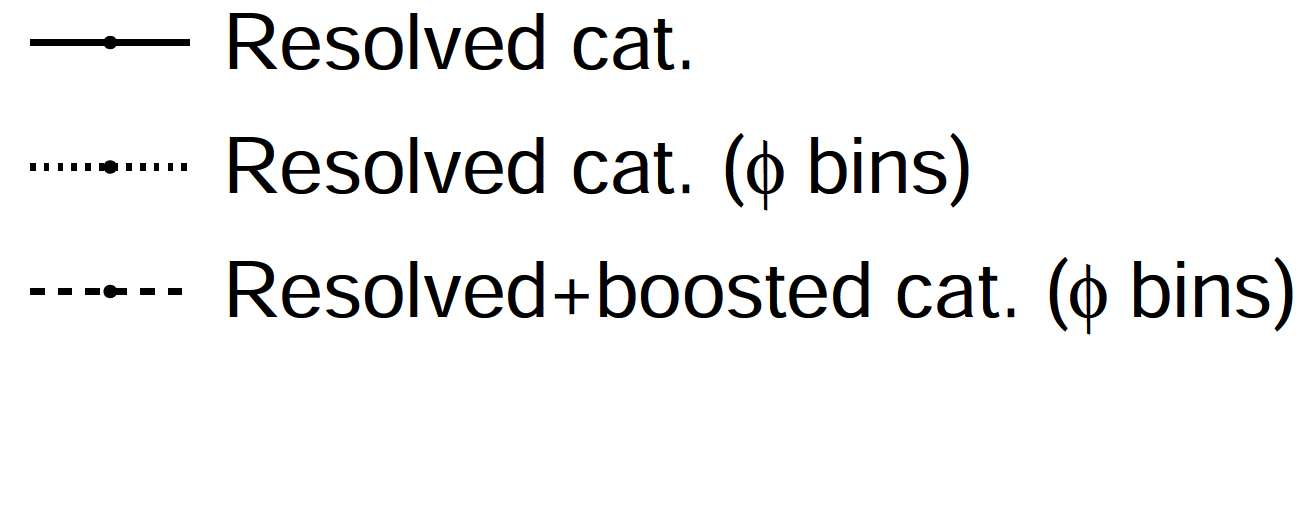
\includegraphics[width=0.495\textwidth]{Figures/RECO/Selection_270.png}
\end{center}
\caption{
Variation of the profile likelihood ratio $q = -2\log\frac{L(\vec{\alpha},\vec{\theta})}{L(\hat{\vec{\alpha}},\hat{\vec{\theta})}}$, where $\vec{\alpha}$ and $\vec{\theta}$ denote parameters of interest and nuisance parameters, respectively, as a function of Wilson coefficients corresponding operators ${\cal O}^{(3)}_{Hq}$ (left), ${\cal O}_{HW}$ (middle), and ${\cal O}_{H\tilde{W}}$ (right) for an integrated luminosity of 300\fbinv.
}
\label{fig:NLL}
\end{figure*}
Fig.~\ref{fig:NLL} shows that a large gain in sensitivity is obtained by adding the boosted category due to the energy growth induced by the operators:
%FIXME: We're not yet saying in the beginning that we solve energy growth with the boosted category!! <-- Yet to be done
The Wilson coefficient corresponding to ${\cal O}^{(3)}_{Hq}$ can be constrained to percent level and the ones corresponding to ${\cal O}_{HW}$ and ${\cal O}_{H\tilde{W}}$ within tens of percent at 95\% confidence level with luminosity amounting to 300\fbinv. 
Quantitative bounds are presented in Table~\ref{Tab:Limits} at 68\% confidence level.
{\renewcommand{\arraystretch}{1.3}
\begin{table}[htbp]
\caption{Expected bounds at 68\% confidence level on Wilson coefficients corresponding to three operators involved in $\PW\PH$ production for integrated luminosity of 300\fbinv.}
\begin{tabular}{lcl lcl lcl lcl}
\multirow{2}{*}{Operator} &
     \multicolumn{3}{c}{Analysis cateogory} \\
    & Resolved & Resolved w/ $\phi$ bins & Resolved+boosted w/ $\phi$ bins \\
    ${\cal O}^{(3)}_{Hq}$    & $\left[-0.16,+0.11\right]$   & $\left[-0.1,+0.08\right]$  & $\left[-0.05,+0.04\right]$ \\
	${\cal O}_{HW}$          & $\left[-0.80,+0.62\right]$   & $\left[-0.78,+0.46\right]$  & $\left[-0.38,+0.26\right]$ \\
	${\cal O}_{H\tilde{W}}$  & $\left[-0.24,+0.22\right]$  &  $\left[-0.22,+0.16\right]$  & $\left[-0.08,+0.06\right]$ \\
  \end{tabular}
\label{Tab:Limits}
\end{table}
% Without the boosted category ... %FIXME <- Quantify the gain! --> Done
An improvement due to a binning in $\phi$ is obtained in the resolved category. 
Simulaneous use of information about all three angles $\Theta$, $\theta$, $\phi$ is expected to result in a large increase in sensitivity. 
%FIXME Let us discuss this statement in person. Is phi weighted with sinxsin? 

\subsection{Possible extensions of ideas}

Here, the proposal is to probe SM-EFT operators in \VH production, where \PV decays to leptons. 
But, the methodology developed also holds for hadronically decaying \PV; 
the only bottleneck in the case of {\PV}$ ={\PW}$ in sensitivity is the absence of knowledge on \PV charge. 
Latest developments in DNN-based methods for vector boson tagging can be used to increase the sensitivity. 

Technologies developed for the proposed measurement can also be directly applied to searches with \PV$\to \Pl^{+}\Pl^{-} / \Pl \Pgn$ and $\PH \to \Pb \PAb$ in the final state, particularly in the context of a heavy resonace decaying to \PV and {\PH}.


\section{Planned cooperation arrangement} 

The work will be conducted within the CMS Collaboration. The reconstructed and simulated data, trigger information, object calibration factors provided centrally by the Collaboration will be used. 
Ideas and updates will be presented at regular intervals in internal meetings. 
In general, no cooperative arrangement is planned for this proposal. 

However, there are synergies with ongoing activities within the CMS data analysis group at HEPHY. 
The group recently submitted a paper on measurement of $\Pt\PAt\Pgg$ process and constraining $\Pt-\Pgg$ coupling in SM-EFT; this work was supported by FWF grant P31578.
There is also ongoing work on constraining SM-EFT operators in $\Pt\PW\PZ$ process supported by FWF grant P33771. 
Thus the proposed measurement will add a complementary direction in terms of the group's activities.

The CMS data analysis group at HEPHY consists of five staff scientists, three post-doctoral researchers, and five Ph.D. students working on supersymmetry, long-lived signatures, search for BSM Higgs boson decaying to a pair of $\tau$ leptons, top quark physics, among others. 
Diverse experience in the group helps to develop new ideas and implement those in the CMS Collaboration.

\section{Work and plan}

The work will be carried out by a new Ph.D. student along with the applicant. 
Since the proposed work is on Higgs physics, which is one of the main centers of activities at LHC, the  
Ph.D. student will get high visibility within the CMS Collaboration.  

Tasks in chronological order are described in the following and summarized in Table~\ref{tab:workplan}.%Fig.~\ref{fig:workplan}.

\begin{enumerate}

\item Signal simulation for Run~2:

The proposed study requires the simulation of \VH events, including the effects of SM-EFT operators both at the levels of production and decay using recently developed software packages, e.g., SMEFTsim~\cite{Brivio:2020onw} at leading-order or using SMEFT@NLO~\cite{Degrande:2020evl} at next-to-leading order in perturbative QCD. 
Particular care needs to be taken for the matching of generation of the hard process using {\MGvATNLO}~\cite{Alwall:2014hca} and the parton shower with PYTHIA8~\cite{Sjostrand:2014zea} 
since the parton shower does not involve higher-dimensional operators. 

\item SM-EFT parameterization:

Information about SMEFT operators will be simulated using a second-order polynomial in the Wilson coefficients involved. A number of weights will be stored for each event. 
It needs to be checked if a second-order polynomial is sufficient to parameterize the effects of SM-EFT operators.

\item Optimization of lepton selection:

The conditions used for lepton identification needs to be optimized in such a way that the variation of acceptance for different operators and the total systematic uncertainty are minimized while not compromising on the statistical power of data. 

\item Optimization of \Pb tagging condition: 

The CMS Collaboration provides the correction to be applied to simulation to match the efficiency of DNN-based \Pb in data and simulation in two variants. 
The first one, the working point-based method, requires to use certain pre-defined thresholds on \Pb tagging score of a jet to qualified a 'b-tagged' and the corresponding correction has smaller uncertainties. 
In the second approach, the shape-based method, one can put the threshold at any value in \Pb tagging discriminator and the corrections have larger uncertainties. Since the \Pb tagging information is used for signal-to-background discrimination, it needs to be checked which of the two options provides better overall sensitivity.  

\item Optimization of \PH tagging condition and calculation of correction:

The threshold on the DNN-based \PH tagging condition needs to be optimized since this is required for signal-to-background separation. 
Correction factors need to be appropriately calculated to match the tagging efficiency in data and simulation.

\item Trigger efficiency measurement:

The efficiency of lepton-based triggers needs to be measured in both data and simulation. 
Corrections to match the trigger simulation and data will be derived and applied to the simulation. 
The same needs to be performed for the backup jet triggers. 

\item Neutrino reconstruction:

A careful analysis is required to assign the correct $\eta$ to the neutrino, which also benefits the CP-sensitivity of the measurements in case of $\PW\PH$ production. 
A powerful prescription developed for neutrino reconstruction will also help similar analyses ongoing in CMS. 

\item Background estimation:

In the proposed measurement, the backgrounds are primarily planned to be taken from simulation with a thorough validation by comparing those with data in dedicated control regions. 
Corrections need to be derived wherever needed, and the corresponding systematic uncertainties need to be quantified.   

\item Multivariate analysis: 

Modeling of the variables used for signal-to-background separation in DNN-based multivariate analysis and their correlations need to be properly checked. 
The architecture of the DNN and the threshold of the MVA discriminator need to be optimized. 
The modeling of the MVA discriminator for different background processes will be checked, 
and data-to-simulation corrections will be derived if needed. 

\item SM-EFT to SM separation: 

In the feasibility study, the constraints on Wilson coefficients are derived just by separating events in different regions. A more sophisticated study with larger number of variables and taking into account their correlation needs to be used. 
This will be a test-bed of a method proposed by the group at HEPHY using boosted decision trees~\cite{Chatterjee:2021nms}. 

\item Experimental systematic uncertainties: 

Systematic uncertainties related to different objects, e.g. leptons, jets and corrections at event-level need to be applied. The systematic uncertainties need to be properly derived for the corrections developed during this particular analysis. 

\item Modeling uncertainties: 

Modeling uncertainties in simulation from the choice of renormalization and factorization scales, parton distribution function, parton shower need to be derived and applied to all the predictions taken from simulation. 
The neutrino reconstruction is also expected to be affected by the modeling uncertainties. 

\item Quantification of sensitivity: 

Results from different years of Run~2 will be combined and
the sensitivity of the analysis will be quantified using likelihood scans, taking into account correlation between the operators. 
The correlation between systematic uncertainty sources in different years needs to be properly defined. 
It will be carefully checked if some of the systematic uncertainties are unexpectedly constrained. 

\item SM-EFT effects in the background:

So far, all the discussions regarding the SM-EFT operators are made for \VH production, which is the signal targeted. However, some of the operators in Table~\ref{Tab:Operators} also affect some of the background processes. 
For example, ${\cal O}^{(1)}_{Hq}$, ${\cal O}^{(3)}_{Hq}$ affect the diboson production, which is related to \VH production by Goldstone boson equivalence theorem at high energy. 
These are also expected to affect {\PV}+jets production. 
A significant amount of effort needs to be dedicated to the simulation of SM-EFT effects for the backgrounds, followed by a joint analysis of signal and background to report the final sensitivity to the corresponding Wilson coefficients. 

\item Publication based on Run~2 data:

A first paper will be written reporting the results based on Run~2 data. This involves a series of reviews within the CMS Collaboration and finally by the journal reviewers. 

\item Signal simulation for Run~3:

The setup developed for the signal simulation for Run~2 will be used in Run~3. However, options will be kept open to incorporate the developments in the theory community by this period. 

\item Trigger efficiency measurement and optimization of object selection for Run~3: 

The triggers which were operational during Run~2 are expected to be available for Run~3 also, but the pileup condition is likely to change. So, the trigger efficiency and corresponding corrections need to be also derived for Run~3. 
For the same reason, object selection criteria need to be reevaluated for Run~3. 

\item Choice of \PH tagger for Run~3:

With the fast progress in heavy particle tagging, more powerful taggers are expected to be available during Run~3 schedule. An evaluation will be performed based on the available taggers, and the best performant one will be used. 

\item Background estimation for Run~3:

Improvements are expected in the Monte Carlo simulation of different processes in the next few years. Thus, the background estimation strategy to be developed for Run~2 analysis will need validation for Run~3.

\item Experimental and modeling systematic uncertainties for Run~3:

Systematic uncertainties due to experimental sources will be added. Modeling uncertainties are expected to be very similar to Run~2.

\item Combination of Run~2 and~3 results:

Results from the analyses based on Run~2 and Run~3 datasets will be combined. Final sensitivity on Wilson coefficients will be reported based on the combined dataset. 

\item Publication of final results:

The final results will be reported in a paper, which will go through the internal review process by the CMS Collaboration and finally be submitted to the journal for publication. 

\end{enumerate}
\begin{sidewaystable}[ht]
\small
  \begin{tabular}{l|c|c|c|c|c|c|c|c|c|c|c|c|c}
    \multirow{2}{*}{Task / Year} &
      \multicolumn{4}{c|}{2022 ($\int \mathcal{L}dt \sim 30$\fbinv)}  &
      \multicolumn{4}{c|}{2023 ($\int \mathcal{L}dt \sim 120$\fbinv)}  & 
      \multicolumn{3}{c|}{2024 ($\int \mathcal{L}dt \sim 160$\fbinv)} \\
    & Jan-Mar & Apr-Jun & Jul-Sep & Oct-Dec & Jan-Mar & Apr-Jun & Jul-Sep & Oct-Dec & Jan-Mar & Apr-Jun & Jul-Dec \\
    \hline
    1. Signal simulation for Run~2 & \textcolor{orange}{\checkmark} &  &  &  &  &  &  &  &  &  &     \\
    2. SM-EFT parameterization & \textcolor{blue}{\checkmark} &  &  &  &  &  &  &  &  &  &     \\
    3. Optimization of lepton selection &  & \checkmark & & & &  &  &  &  &  &     \\
    4. Optimization of \Pb tagging condition &  & \checkmark & & & &  &  &  &  &  &     \\
    5. Optimization of \PH tagging condition  &  & \checkmark & & & &  &  &  &  &  &     \\
    6. Trigger efficiency measurement &  &  & \textcolor{blue}{\checkmark} & & &  &  &  &  &  &    \\
    7. Neutrino reconstruction  &  & & \textcolor{blue}{\checkmark} & & & &  &  &  &  &     \\
    8. Background estimation &  &  &  & \checkmark & & &  &  &  &  &     \\
    9. Multivariate analysis &  &  &  & \textcolor{blue}{\checkmark} & & &  &  &  &  &      \\
    10. SM-EFT to SM separation &  &  & & & \textcolor{orange}{\checkmark} & & &  &  &  &       \\
    11. Exp. systematic uncertainties  &  &  &  &  & \checkmark & &  &  &  &  &      \\
    12. Modeling uncertainties &  & &  &  & \checkmark & & &  &  &  &       \\
    13. Quantification of sensitivity &  & & & & & \textcolor{blue}{\checkmark} & &  &  &  &      \\
    14. SM-EFT effects in background & &  & & & & \textcolor{orange}{\checkmark} & &  &  &  &     \\
    15. Publication based on Run~2 data &  & & & & &  &  & \textcolor{blue}{\checkmark} &  &  &       \\
    16. Signal simulation for Run~3 &  &  & & & &  & \checkmark & &  &  &      \\
    17. Selections for Run~3 & &  & & & &  & \textcolor{blue}{\checkmark} & &  &  &       \\
    18. Choice of \PH tagger for Run~3 &  & & &  &  &  &  &\checkmark  &  &  &      \\    
    19. Background estimation for Run~3 &  & & &  &  & &  & \textcolor{blue}{\checkmark} & &  &      \\
    20. Systematic uncertainties for Run~3 &  & &  &  & &  &  &  & \checkmark &  &      \\
    21. Combination of Run~2 and~3 results &  & & &  &  &  &  &  &  & \textcolor{blue}{\checkmark}  &      \\
    22. Publication of final results &  & & &  &  &  &  & &  &   & \textcolor{blue}{\checkmark}    \\
  \end{tabular}
  \caption{
Tasks shown using symbol \checkmark will be covered by the Ph.D. student, \textcolor{blue}{\checkmark} by the project applicant and Ph.D. student, \textcolor{orange}{\checkmark} by the project applicant and Ph.D. student in collaboration with other members in HEPHY CMS data analysis group.
}
\label{tab:workplan}
\end{sidewaystable}


\section{Ethical, safety-related or regulatory aspects}

The sole aim of the project is to improve the human understanding of nature. 
The topic itself has no ethical, safety-related, or regulatory aspects that need to be considered.

\section{Sex-specific and gender related issues}

The sole aim of the project is to improve the human understanding of nature. 
Thus the topic itself does not have any gender-related aspects. 
The job advertisement will be formulated gender neutrally. 
In order to improve the gender balance at HEPHY
($\sim 20\%$), a suitable female candidate will be given preference.

\section{Human resources}

A Ph.D. student will be recruited solely for this project to be conducted at HEPHY, Vienna. 
The Ph.D. student will carry out the project under the supervision of the project applicant, PI Dr. S. Chatterjee. 
According to the plan, the PI will spend $50\%$ of his time for this project. 
The PI has five years of experience in CMS data analysis in the context of precision jet measurements, searches for new physics, detector calibration, and implementation of algorithms in the CMS software framework. 
The PI has also worked on high energy physics phenomenology in collaboration with professional theorists and published papers in international journals. 

Tasks will be carried out in consultation with the leader of CMS data analysis group of the institute: Dr. Robert Sch{\"o}fbeck (RA), who is also performing SM-EFT measurements in top quark physics in association with a post-doctoral researcher Dr. Dennis Schwartz (DS). Cross-talk with RA and DS will be extremely useful for this project. 
Particularly, the simulation of SM-EFT operators (task 1), SM-EFT parameterization (task 2), and SM-EFT to SM separation (task 10) will be performed together with RA and DS. 
RA is also the former convener of the 'top quark mass and properties' physics analysis group and the 'jet and MET' physics object group of the CMS Collaboration. 
His feedback on documentation and presentation of the results will be constructive. 

\appendix
\renewcommand{\thesection}{Annex \arabic{section}} 
\addtocontents{toc}{\setlength{\cftsecnumwidth}{11ex}}

\clearpage
\section{References}
\renewcommand{\refname}{}
{
%\bibliographystyle{jhep}
\bibliographystyle{lucas_unsrt}
\bibliography{VHeft}
}

\newpage

\section{Research institution and required funding}

The Institute of High Energy Physics (HEPHY) of the Austrian Academy of Sciences was founded in 1966. 
Its main purpose is the research in high energy physics and to exploit Austria's membership at CERN. 
On the hardware side, HEPHY has made significant contributions to the CMS inner tracker and to the trigger system. 
The CMS data analysis group, led by Dr. R. Sch{\"o}fbeck, consists of 14 members based at offices in the Apostelgasse 23 in Vienna and at CERN. The successful candidate will be based in Vienna. 
This choice will enable a direct collaboration with the other Ph.D. students and two master students doing data analysis in CMS, as well as with the scientist of the New Physics theory group.
Additionally, four members are based at CERN. 
Among them is Dr. W. Adam, the former physics coordinator of the CMS experiment and the leader of HEPHY team at CERN.

The infrastructure available to the HEPHY CMS analysis group comprises:
\begin{itemize}
\item Office space with personal workstations at Apostelgasse 23.
\item Access to an LHC-Grid (LCG) Tier-2 cluster with 1000 CPU cores and 500 TByte storage. Access to the CLIP computing cluster at the Gregor Mendel Institute of the Austrian Academy of sciences with approx. 10k CPU cores and 50 TB of
storage for analysis work.
\item Video-conferencing equipment for daily communication with other CMS physicists and for participation in meetings in the CMS collaboration.
\end{itemize}

This project application requests funding for one Ph.D. student for 36
months (EUR 39.780 per year in 2021). 
The PI S. Chatterjee is a post-doctoral researcher at HEPHY.
Upon a positive funding decision by the FWF, a call for the Ph.D. student will be opened, advertised inside and outside Austria, and made equally accessible to physicists regardless of their race, color, creed, national origin, religion, family status, sexual orientation, age, and political beliefs. 
In order to improve the gender balance at HEPHY ($\sim 20\%$), a suitable female candidate will be given preference.

Furthermore, a total of EUR 5.155 per year for travel expenses between Vienna and CERN is requested. 
These costs are justified as follows: 
The Ph.D. student will travel four times a year (approximately every two months) to CERN for, on average, one week.
The purpose of four trips is the collaboration with the other experimentalists in the CMS HIG group and to present in person to the other members of the CMS collaboration.
Also, the Ph.D. student will get an opportunity to participate in the detector operation during the data-taking periods. 
If possible, the CERN trips will overlap with a CMS collaboration week (internal CMS working meeting occurring four
times a year at CERN). 
Furthermore, one trip to the annual Higgs conference is foreseen, where recent developments in experimental and theoretical results on the Higgs boson are presented. 
Cost for this trip is assumed to be the same as for a trip to CERN.
A breakdown of the expected costs of a working travel to CERN is provided in Table~\ref{Tab:Travel_cost}. 
\begin{table}
\caption{Estimation of travel costs for trips to CERN.}
\begin{tabular}{m{5 cm}| m{4 cm}| m {4 cm}}
Item & Cost & Comment \\
\hline 
Flight VIE-GVA-VIE & EUR 300 & \\
7 per diem at EUR 28,10 & EUR 196,70 & \\
7 per noctem at EUR 24,90 & EUR 174,30 & \\
6 hotel nights at EUR 60 & EUR 360  & \\
\hline
Total per year & EUR 5.155 & 5 trips per year \\
\hline
Total & EUR 15.465 & For 3 years in total
\end{tabular}
\label{Tab:Travel_cost}
\end{table}

The institute needs to pay an amount (MoE) for the PI, which amounts to EUR 10.000 per year, 
this is also requested in the proposal.
An extra $5\%$ of the total that amounts to EUR 164805 is requested to cover other unexpected costs.  
Total requested funding sums up to EUR 173045.  
A summary of the total costs of the project is provided in Table~\ref{Tab:Total_cost}.
\begin{table}
\caption{Total amount of requested funding.}
\begin{tabular}{m{6 cm}| m{4 cm}}
Item & Cost  \\
\hline 
Ph.D. student's salary & EUR 119340  \\
Ph.D. student's travel costs of & EUR 15465 \\
MoE of the PI (for 3 years) & EUR 30000 \\
\hline
General costs ($5\%$) & EUR 8240  \\
\hline
Total & EUR 173045 
\end{tabular}
\label{Tab:Total_cost}
\end{table}

\newpage


\section{CV of the principal investigator}

\subsection*{\underline{Personal Data}}

\textbf{Age:} 27 years (as of February 1, 2021)\\
\textbf{Nationality:} Indian \\
\textbf{Sex:} Male \\
\textbf{Affiliation:} Institute of High Energy Physics (HEPHY), Vienna \\
\textbf{Designation:} Post-doctoral researcher 

%\textbf{Ph.D. Supervisor:} \\ Prof. Gobinda Majumder, \\ Department of High Energy Physics, \\
%Tata Institute of Fundamental Research, Mumbai \\

\subsection*{\underline{Contact Details}}

\textbf{Email:} s7384705218@gmail.com, suman.chatterjee@cern.ch\\
\textbf{Phone: } +91-7710835260, +43-6769394076\\
\textbf{Website: } \href{https://sumanchatterjeetifr.wordpress.com}{https://sumanchatterjeetifr.wordpress.com}


\subsection*{\underline{Academic Records}}

\textbf{2016-2020:}
Ph.D. in Experimental Particle Physics\\
Department of High Energy Physics\\
Tata Institute of Fundamental Research, Mumbai 400005\\
Degree awarded in August 2020
\\
\\
\textbf{2014-2016:}
Master of Science in Physics\\
Tata Institute of Fundamental Research, Mumbai 400005\\
Rank: 1st
\\
\\
\textbf{2011-2014:}
Bachelor of Science in Physics\\
Department of Physics\\
Jadavpur University, Kolkata  700032\\
Remark: 1st class

\subsection*{\underline{Achievements}}

\begin{tabular}{ p{2cm} p{13cm} }
\textbf{2020} & {Received \textbf{Honorable mention} for the \textbf{IPA Rahul Basu Memorial Award for Best Thesis in High Energy Physics} for the period 2018--2020 in XXIV DAE-BRNS HEP Symposium 2020, India} \\
\textbf{2015} & {Awarded \textbf{Professor Sukumar Biswas Ph.D. Student Award for Excellence in Physics} for scoring the highest grades in graduate courses in the Physics Integrated Ph.D. program in Tata Institute of Fundamental Research} \\
\textbf{2015} \ & Qualified CSIR-UGC National Eligibility Test in Physics with \textbf{All India Rank 43} \\
\textbf{2014} \ & Secured \textbf{All India Rank 3} with 99.63 percentile in Joint Entrance Screening Test 2014 conducted by the research institutes in India  \\
\textbf{2011-2014} \ &  Awarded \textbf{INSPIRE SCHOLARSHIP} by Department of Science and Technology, India for being within top 1\% students appeared from West Bengal Board of Higher Secondary Education in Higher Secondary (10+2) Examination \\
\textbf{2011} \ & Awarded by the Chief Minister of the state of West Bengal for securing \textbf{the 4$^{\rm{th}}$ rank in the State} in Higher Secondary (10+2) Examination (conducted by West Bengal Council for Higher Secondary Education)  \\
\end{tabular}


\begin{comment}
\subsection*{\underline{CMS Internal Notes \small{(excluding the notes corresponding to the papers)}}}

\textbf{1:} \textit{BSM H$\to \tau\tau$ analysis on full Run~2 CMS data at $\sqrt{s}=$ 13\,TeV}\\
\ CMS-AN-2020-218\\
\textit{Search for additional Higgs bosons predicted by supersymmetry in the case where the Higgs boson decays to a pair of $\tau$ leptons}\\
\\
\textbf{2:} \textit{Electronic top tagger in CMS}\\
%Suman Chatterjee, Debarati Roy, and Gobinda Majumder \\
\ CMS-AN-2020-168\\
\textit{Implementation and performance monitoring of the algorithm developed in JHEP 01 (2020) 170 in CMS experiment}\\
\\
\textbf{3:} \textit{Implementation of recursive soft drop algorithm in CMS software, and performance studies}\\
%Suman Chatterjee, and Gobinda Majumder \\
\ CMS-AN-2018-070\\
\textit{Implementation of a new jet grooming algorithm, named `recursive soft drop' (JHEP 06 (2018) 093) in CMS software framework and monitoring its performance at HL-LHC}\\
\end{comment}
%\textbf{3:} \textit{Radius scan for inclusive jets in CMS experiment}\\
%Suman Chatterjee, and Gobinda Majumder \\
%\ CMS-AN-2018-044\\

%\textbf{4:} \textit{Upgrade of HO weight factor in particle-flow algorithm}\\
%Suman Chatterjee, and Gobinda Majumder \\
%CMS-DN-2016/023\\


\subsection*{\underline{Oral Presentations at Conferences, Workshops}}

\textbf{September 2021} \ \textbf{Joint annual meeting of Austrian and Swiss physical societies, Innsbruck, Austria} \\
Parallel talk \\
SM-EFT results in Higgs sector from the CMS experiment\\
\\
\textbf{July 2021} \ \textbf{European Conference on High Energy Physics (EPS-HEP 2021), Hamburg, Germany (online)} \\
Parallel talk \\
Jet substructure measurements in CMS\\
\\
\textbf{Dec 2020} \ \textbf{XXIV DAE-BRNS HIGH ENERGY PHYSICS SYMPOSIUM 2020} \\
Rahul Basu Memorial Thesis Award Seminar \\
Jets as probes for precision measurement and candles for physics beyond standard model\\
\\
\textbf{Jan 2020} \ \textbf{QCD with Electron-Ion Collider (QEIC), IIT Bombay, Mumbai, India} \\
Plenary talk (on behalf of ATLAS, CMS, and LHCb Collaborations) \\
Understanding parton distribution function from LHC measurements\\
\\
\textbf{Sep 2019} \ \textbf{Workshop on Top Quark Physics (TOP2019), IHEP, Beijing, China} \\
Invited talk (on behalf of ATLAS and CMS Collaborations) \\
Heavy resonance searches in ATLAS and CMS \\
\\
\textbf{July 2019} \ \textbf{European Conference on High Energy Physics (EPS-HEP 2019), Ghent, Belgium} \\
Parallel talk (on behalf of CMS Collaboration) \\
Inclusive jet results from CMS experiment  \\
\\
\textbf{July 2019} \ \textbf{European Conference on High Energy Physics (EPS-HEP 2019), Ghent, Belgium} \\
Parallel talk \\
Tagging top in leptonic decay \\
\\
\textbf{Feb 2019} \ \textbf{International Workshop on Forward and Jet Physics at LHC, Bose Institute, Kolkata, India} \\
Invited talk (on behalf of CMS Collaboration) \\
Measurement of inclusive jet cross section and event properties in CMS experiment \\
\\
\textbf{Aug 2018} \ \textbf{QCD at LHC 2018, Technische Universit{\"a}t Dresden, Dresden, Germany} \\
Parallel talk (on behalf of ATLAS, CMS, and LHCb Collaborations) \\
Top quark and jet measurements sensitive to PDFs  \\
\\
\textbf{Aug 2018} \ \textbf{QCD at LHC 2018, Technische Universit{\"a}t Dresden, Dresden, Germany} \\
Parallel talk (on behalf of CMS Collaboration) \\
Differential jet cross sections at the CMS experiment \\
\\
\textbf{Dec 2017} \ \textbf{Workshop on High Energy Physics Phenomenology XV, IISER Bhopal, Bhopal, India} \\
Parallel talk (on behalf of CMS Collaboration)\\
Radius Scan for Inclusive Jets in CMS Experiment at $\sqrt{s} =$ 13\,TeV \\
\\
\textbf{Dec 2016} \ \textbf{XXII DAE-BRNS High Energy Physics Symposium, Delhi, India} \\
Parallel talk (on behalf of CMS Collaboration) \\
Perspectives for a Radius Scan in Inclusive Jets at 13\,TeV with CMS  \\

\subsection*{\underline{Poster Presentations}}

\textbf{June 2021} \ \textbf{Large Hadron Collider Physics (LHCP 2021) conference, Paris, France (online)}\\
Search for W$^{\prime}$ bosons decaying to a top and a bottom quark at $\sqrt{s}=$ 13\,TeV\\
\\
\textbf{Sep 2018} \ \textbf{Asia-Europe-Pacific School on High Energy Physics, Quy Nohn, Vietnam}\\
Radius scan for inclusive jets at $\sqrt{s}=$ 13\,TeV\\
\\
\textbf{Dec 2016} \ \textbf{XXII DAE-BRNS High Energy Physics Symposium, Delhi, India}\\
HO weight factor in particle flow algorithm in CMS\\

\subsection*{\underline{Teaching Experience}}

\textbf{Autumn 2019: Teaching assistant}\\
Course: Statistical Methods in Physics\\
Instructor: Prof. G. Majumder, TIFR\\
\\
\textbf{January 2019: Co-coordinator}\\
Software session (lecture and hands-on exercise on algorithms used in high energy physics for event generation, object reconstruction, and analysis) 
at the XII School on Experimental High Energy Physics conducted by the Science and Engineering Research Board in India \\
\\
\textbf{Autumn 2016: Teaching assistant}\\
Course: Electrodynamics II\\
Instructor: Prof. G. Ravindra Kumar, TIFR\\

\subsection*{\underline{Supervision Experience}}

\textbf{Anirban Bala} (Ph.D. student at TIFR, Mumbai, Advisor: Prof. Monoranjan Guchait):\\
During his departmental project I (July-September, 2020) under Prof. Gobinda Majumder at TIFR \\
Designed the project and mentored thoroughly during its implementation\\

\subsection*{\underline{Organizational Responsibilities}}

\textbf{XII School on Experimental High Energy Physics} at TIFR, Mumbai\\
Helped the organization at the institute level\\
\\
\textbf{SUSY 2017} conference at TIFR, Mumbai\\
Led the team of volunteers \\

\newpage

\section*{{Selected Publications}}

\textbf{1:} \textit{
Search for a W$^\prime$ boson decaying to a top and a bottom quark at $\sqrt{s}=13$\,TeV}\\
CMS Collaboration \\
Phys. Lett. B 820 (2021) 136535 \\
\textit{Most stringent limits published to date on right- and left-handed W$^\prime$ bosons decaying to a top and a bottom quark.}\\
\\
%\textbf{2:} \textit{
%Tree boosting for learning EFT parameters}\\
%arXiv:2107.10859\\
%\textit{A new tree boosting algorithm designed for the measurement of parameters in the context of effective field theory.}
%\\
\textbf{2:} \textit{
Dependence of inclusive jet production on the anti$\mbox{-}k_T$ distance parameter in pp collisions at $\sqrt{s} = 13$\,TeV}\\
CMS Collaboration \\
JHEP 12 (2020) 082\\
\textit{First public results from colliders on dependence of inclusive jet cross section on jet size.}\\
\\
\textbf{3:} \textit{Calibration of the CMS hadron calorimeters using proton-proton collision data at $\sqrt{s}= 13$\,TeV}\\
CMS Collaboration \\
JINST 15 (2020) P05002\\
\textit{Absolute calibration of outer hadron calorimeter in particle-flow algorithm in CMS.}\\
\\
\textbf{4:} \textit{Jets with electrons from boosted top quarks}\\
Suman Chatterjee, Rohini Godbole, and Tuhin S. Roy\\
JHEP 01 (2020) 170\\
\textit{An algorithm to identify boosted top quarks decaying where W boson from top quark decays to an electron using jet substructure techniques.}\\
\\
\textbf{5:} \textit{Mixed WIMP-axion dark matter}\\
Suman Chatterjee, Anirban Das, Tousik Samui, and Manibrata Sen\\
Phys. Rev. D 100, 115050\\
\textit{A detailed study of the phenomenology of a multi-component dark matter scenario with
a scalar WIMP and the QCD axion in the light of the latest data from dark matter detection experiments and
LHC results.}\\
\\
%\textbf{7:} \textit{Les Houches 2017: Physics at TeV Colliders Standard Model Working Group Report}\\
%arXiv:1803.07977 \\
%\textit{A detailed study of two-prong taggers and measurement of strong coupling using jet substructure}
%\\
\textbf{6:} \textit{Dose rate effects in the radiation damage of the plastic scintillators of the CMS hadron endcap calorimeter}\\
CMS Collaboration \\
2016 JINST 11 T10004\\
%arXiv:1608.07267\\
\textit{Measurements of change in light output by plastic scintillators in the CMS hadron endcap due to irradiation during the collisions at LHC at $\sqrt{s} = 8$\,TeV.}\\


%------------------------------------------------

\end{document}
